\documentclass{hotnets19}

\usepackage{times}  
\usepackage{hyperref}
\usepackage{listings, multicol}
\usepackage{lipsum}
\usepackage{xcolor}
\usepackage{graphicx}
\usepackage{subcaption}
\usepackage{mdframed}


\usepackage{float}
% \usepackage[export]{adjustbox}

\usepackage{booktabs}

\hypersetup{pdfstartview=FitH,pdfpagelayout=SinglePage}

\setlength\paperheight {11in}
\setlength\paperwidth {8.5in}
\setlength{\textwidth}{7in}
\setlength{\textheight}{9.25in}
\setlength{\oddsidemargin}{-.25in}
\setlength{\evensidemargin}{-.25in}


\definecolor{mygray}{gray}{0.99}
\definecolor{commentcolor}{RGB}{0,100,0}

\lstdefinelanguage{P4}{
  keywords={in, out, inout, function, return, switch, enum, if, else, case, break, extern, void, bit, error, int, verify, bool, key, table, action, actions, parser, control, state, transition, select, apply},
  keywordstyle=\color{blue}\bfseries,
  keywords=[2]{boolean, string, number, objectid},
  keywordstyle=[2]\color{green}\bfseries,
  identifierstyle=\color{black},
  sensitive=false,
  comment=[l]{//},
  morecomment=[s]{/*}{*/},
  commentstyle=\color{commentcolor}\ttfamily,
  stringstyle=\color{red}\ttfamily,
  morestring=[b]',
  morestring=[b]"
}

\lstset{
   language=P4,
%    backgroundcolor=\color{mygray},
   extendedchars=true,
   basicstyle=\small\ttfamily,
   showstringspaces=false,
   showspaces=false,
   tabsize=2,
   frame=single,
   breaklines=true,
   showtabs=false
}


\begin{document}

% \conferenceinfo{HotNets 2019} {}
% \CopyrightYear{2019}
% \crdata{X}
% \date{}

%%%%%%%%%%%% THIS IS WHERE WE PUT IN THE TITLE AND AUTHORS %%%%%%%%%%%%

\title{HotNets 2019 Paper}

\author{Paper \#0, 3 pages}

\maketitle

%%%%%%%%%%%%%  ABSTRACT GOES HERE %%%%%%%%%%%%%%
\begin{abstract}



\end{abstract}

\section{Introduction}

\textbf{TODO: unify the terminology, functions / modules / packages}


Software-Define Networking paradigm provides a great flexibility to control and manage network devices by separating control and data planes.
Using APIs, Control plane can configure objects in data plane at run-time or compile time to achieve desired packet processing behavior or modify it.
Adding into that, P4, a data plane programming language, allows to describe data plane of packet processing logic required to realize a network function and expose APIs to configure the objects the in data plane.
<<1 line on programmable blocks and on re-configurable hardware, Flexpipe, RMT >>

More often, programmers need to describe data and control plane logic of network functions as different programs and in different languages.
This, by design split of logic and execution control flow across multiple heterogeneous programs, increases development, test and deployment complexity of network functions.
Also, it requires novel mechanisms to build complex network functions by reusing independently developed and tested data and control plane code.
However, P4 mandates to write a monolithic data plane program and carefully configure the data plane objects to build a application processing various protocols and performing multiple network functions.
For example, switch.p4~\cite{switch.p4} has control blocks defined to processes different protocol headers and network functions(e.g., l2 switching, l3 routing etc.,). 
But, the control blocks globally share different types of metadata structures and parsed headers. 
Without understanding implementation details of the program, reuse of the code is difficult due to lack of clear interface.
<<Why passing headers to controls as parameters is not good interface?
Explain using innerIP, outer IP, ethernet, vxlan examples that passing headers does not provide unambiguous interface to process packet. 
>>
Existing data plane programming paradigm needs modularity that allow programmers to expose interface to reuse code written to process packet at any granularity of functionalities while abstracting away the implementation details.

Let's consider a simple scenario as shown in Figure~\ref{fig:l3.p4.l2.p4}. A program, l3.p4, parses IPv4 header from packets, performs longest-prefix match and determines next hop. 
Moreover, it decrements the ttl field and deparse the packet. 
Another program, l2.p4, processes the same packet and takes the next hop as input argument, parses Ethernet header, matches on id of next hop and modifies ethernet addresses.
Finally, it deparses the packet and sends on appropriate port.
In this example, l3.p4 is not generating a functionally correct packet to forward on wire. 
However, it can be reused with different layer-2 forwarding mechanism or even with MPLS and create functionally correct packet to forward on wire. 
Similarly, l2.p4 can be reused with IPv6 based routing.
Such fine-grained packet processing modules enable code reuse and modular control over data plane objects, thereby facilitating incremental development of network functions. 

\begin{figure*}
\noindent \begin{minipage}[t]{.48\textwidth}
\begin{lstlisting}[frame=none]
// l3.p4
parser P(packet_in pin, out hdr_t hdrs) {
  state start {
    pin.extract(hdrs.eth);
    transition select(hdrs.eth.ethType){
       0x0800: parse_ipv4;
    }
  }
  state parse_ipv4 {
      pin.extract(hdrs.ipv4);
      transition accept;
  }
}
control Pipe(inout hdr_t hdrs, out bit<16> nexthop_id, inout sm_t sm) {
  action process(bit<16> nh) {
    hdrs.ipv4.ttl = hdrs.ipv4 - 1;
    nexthop_id = nh;// setting out param
  }
  table ipv4_lpm_tbl {
    key = { hdrs.ipv4.dstAddr : lpm } 
    actions = { process; }
  }
  apply {
    ipv4_lpm_tbl.apply();
  }
}
control D(packet_out po, in hdr_t hdrs) {
  apply() {
    po.emit(hdrs.eth);
\end{lstlisting}
\end{minipage}
\hfill\begin{minipage}[t]{.48\textwidth}
\begin{lstlisting}[frame=none]
    po.emit(hdrs.ipv4);
  }
}
// l2.p4
parser P(packet_in pin, out hdr_t hdrs) {
  state start {
    pin.extract(hdrs.eth);
  }
}
control Pipe(inout hdr_t hdrs, in bit<16> nexthop_id, inout sm_t sm) {
  action forward(bit<48> dest_mac, bit<48> src_mac, bit<8> out_port) {
    hdrs.eth.dstAddr = dest_mac;
    hdrs.eth.srcAddr = src_mac;
    sm.out_port = out_port;    
  }
  table forward_tbl {
    key = { nexthop_id : exact } 
    actions = { process; }
  }
  apply {
    forward_tbl.apply();
  }
}
control D(packet_out po, in hdr_t hdrs) {
  apply() {
    po.emit(hdrs.eth);
  }
}
\end{lstlisting}
\end{minipage}
% \vspace*{-10pt}
\caption{Fine-grained packet processing modules - l3.p4  and l2.p4}
\label{fig:l3.p4.l2.p4}
\end{figure*}


Previous work, HyPer4~\cite{Hancock:2016:HUP:2999572.2999607}, HyperV~\cite{8038396} use virtualization to support modularity.
P4Visor~\cite{Zheng:2018:PLV:3281411.3281436} supports testing specific composition operators(A-B and Differential) by merging P4 programs using compiler techniques.
In both approaches, minimal composable unit is a data plane program of a network function(e.g., switching, routing etc.,). 
Hence, it does not allow to incrementally develop and enrich a network function by reusing code to support more protocols.
Also, these approaches lack inter-module communication mechanism(e.g., next hop in above example) except via packets.
Encapsulating customized headers inside the packet may allow such communication, but that would require to know
implementation details of deparser in one module to write complimentary parser in other and vice versa. 

parallel processing -copy semantics


In this paper, we present, a Micro Switch Architecture($\mu$SA) and a compiler, $\mu$P4C, for a logical target to build network functions by reusing fine-grained packet processing code.
% $\mu$SA provides a simplified abstraction for packet processing blocks over real targets' architectures.
$\mu$SA allows define interface to expose code modules as callable P4 packages.
P4 programmers can reuse of the code by invoking the packages interfaces without knowing implementation details of the code.
Using $\mu$P4C, programmers can compile real target specific executable by linking all the $\mu$SA based programs, composing them into a single program.
\begin{itemize}
 \item Compiler Midend to link all the programmable blocks compose them as dictated by their call location in execution-control of the source program.
 \item and transform complete CSA specific P4 program to any target architecture (e.g., v1model of BMV2 or PSA)
\end{itemize}

%  
% Contribution in this paper,
% 
%  P4 programs adhering CSA are translated to other architectures(e.g., v1model, PSA) pertaining to software or hardweare target. 
%  
%  we developed backend and blah blah  
%  
%  
%  Techniques to transform parser and deparser architecture blocks of P4 programs into control-blocks comprising match-action tables.
% Compiler midend to merge packet processing functionality described in other p4 programs.

<<Paper outline para  >> rest of the paper is arranged....



\section{Challenges}
P4 is developed to specify data plane functionality of software or hardware targets (e.g., simple\_\-switch~\cite{simple_switch.md}, TOFINO~\cite{tofino} etc.,) devices.
Target device manufacturer provides an architecture description of data plane along with a P4 compiler for the device.
The architecture source file (e.g., v1model.p4~\cite{v1model.p4} for simple\_switch) contains declaration of a set of pro\-gram\-ma\-ble blocks, their data plane interfaces and the target specific metadata (called intrinsic metadata) and extern functions.
To program the packet processing pipeline of a device, P4 programmers provide implementation of the declared programmable blocks in its architecture file.
Therefore, P4 programs are tightly coupled with architecture of the target devices.


The architecture description of a target specifies data plane pipeline comprising a set of pro\-gram\-ma\-ble and fixed-function blocks, flow of user-defined and target-specific (called intrinsic) metadata in the pipeline and semantics of target-specific actions and externs.
For example, Figure \ref{subfig:psa-model} and \ref{subfig:v1model} show data plane pipelines and their packet processing blocks defined in v1model~\cite{simple_switch.md} and Portable Switch Architecture (PSA) \cite{psa}, respectively.

\begin{figure}
    \begin{subfigure}{\linewidth}
        \centering
        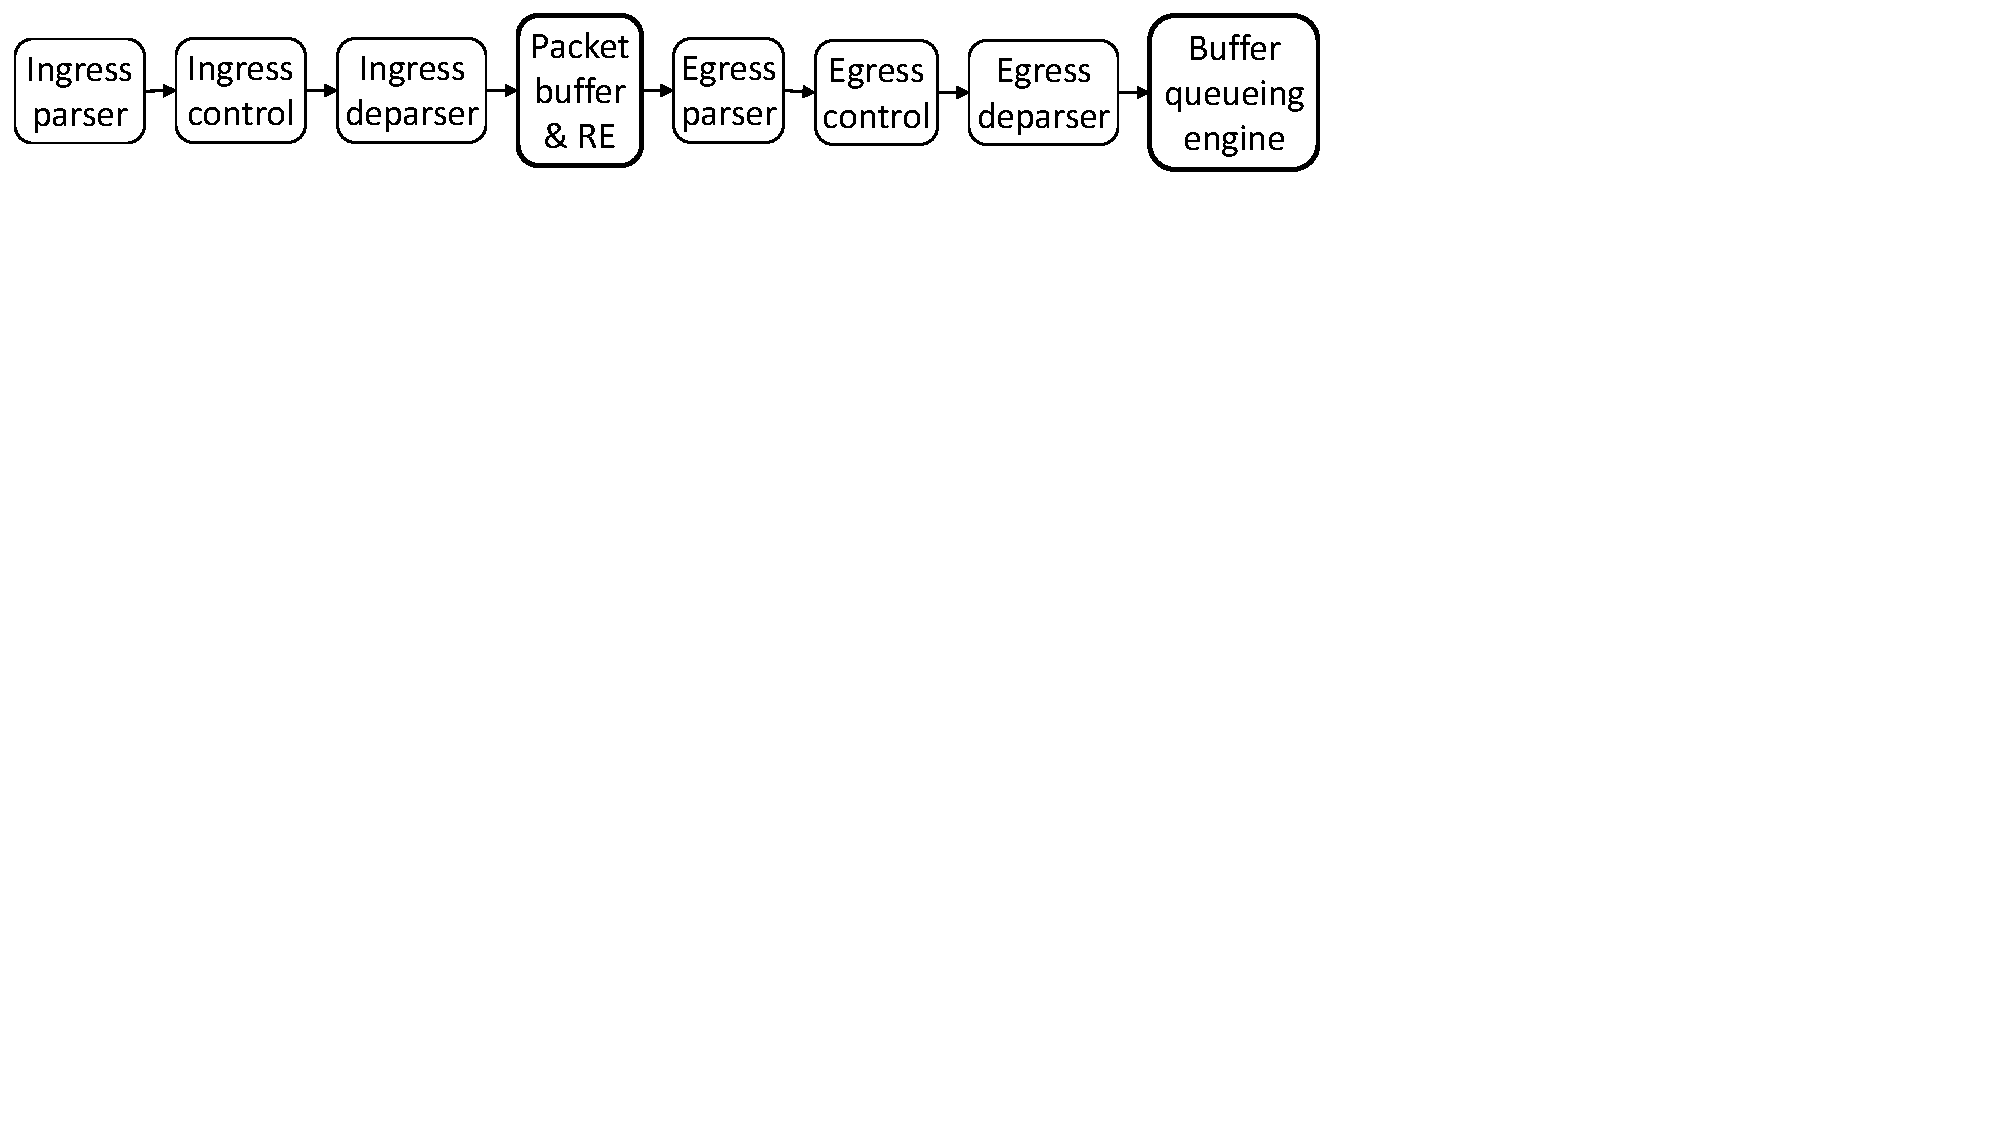
\includegraphics[trim=7 450 281 0, clip,scale=0.36]{psa-pipeline.pdf}
        \caption{PSA Model}
        \label{subfig:psa-model}
    \end{subfigure}
    \begin{subfigure}[b]{\linewidth}
        \centering
        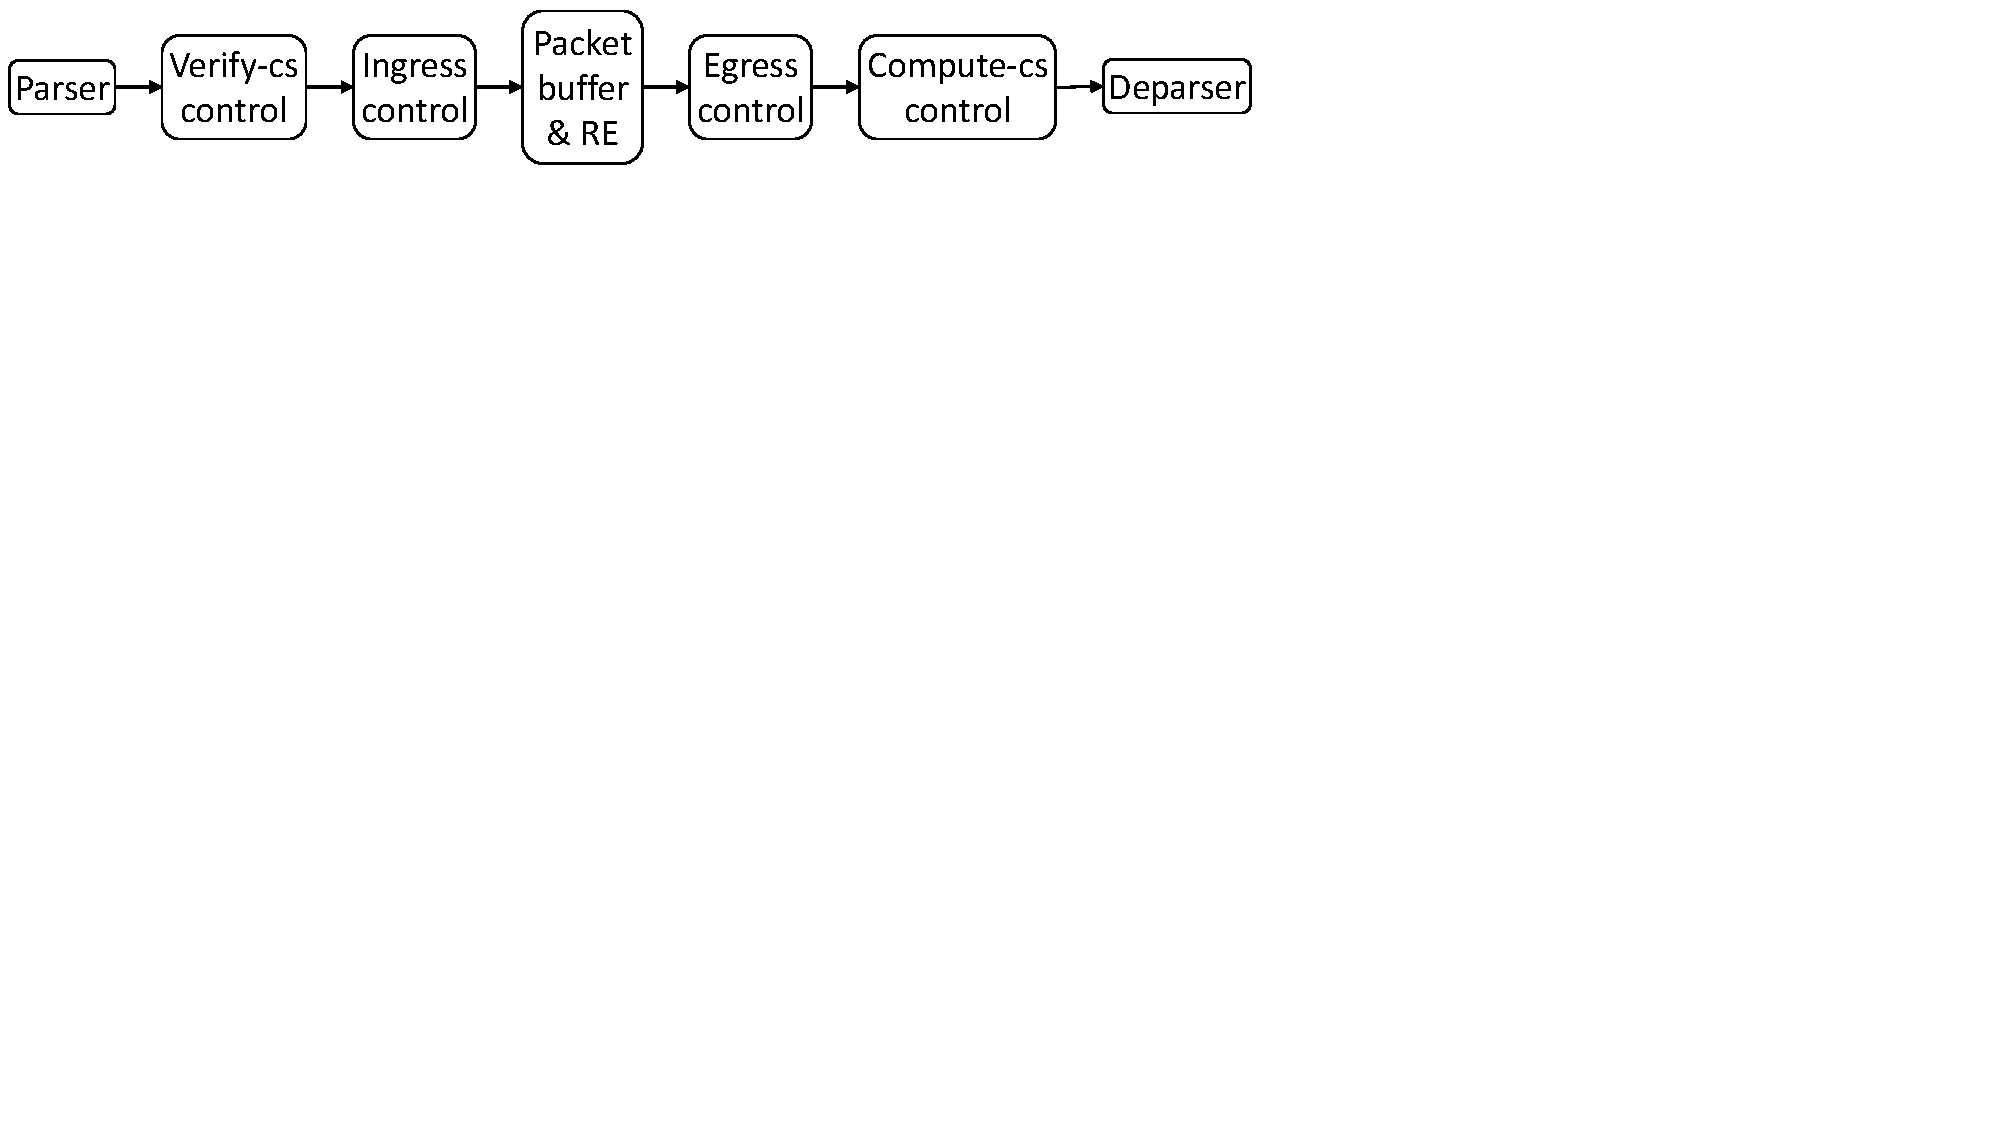
\includegraphics[trim=3 460 357 0, clip,scale=0.35]{v1model-pipeline.pdf}
        \caption{simple\_switch v1 Model}
        \label{subfig:v1model}
    \end{subfigure}
\caption{Real Target Architectures}
\label{fig:real-target-architectures}
\end{figure}


Parser blocks are described using a sub-language of P4, based on abstraction of Finite State Machine.
Control blocks are expressed using a sub-language modelling imperative control flow.
Deparsers are special control blocks that allows to use statements, to reassemble packets, that are prohibited in other control blocks.
Packet processing logic in P4 programs are sectioned across programmable blocks with heterogeneous abstract machines (e.g., parsers, deparsers, control) and fixed-function blocks (Packet Buffer and Replication Engine).
Therefore, a control block can not instantiate and execute parser blocks. Similarly, deparser block can not invoke and execute parser blocks.  
Consider the example in Figure~\ref{fig:l3.p4.l2.p4}, parser ``P'' of l2.p4 can not be executed at the end of deparser control block ``D'' of l3.p4.


Moreover, architectures models expose intrinsic metadata, target-specific actions and extern functions (e.g., resubmit, recirculate, clone) to replicate and/or program packet-path and flow of data across the processing blocks, as described in~\cite{simple_switch.md} and ~\cite{psa}
In turn, adding different abstract-machine to program packet-path and data flow across the blocks and further increasing heterogeneity in the model of a data plane program.
<<For example, resubmit or recirculate calls are like event trigger.. effects happen after the block>>

Finally, the existing architecture models expose target-specific constraints.
E.g., output port can not be changed in egress control block, scope of some intrinsic metadata bounded by particular programmable blocks, etc.,  
Programmers need implement execution logic conforming to constraints, architecture model and semantics of actions and extern functions of the target device.


% P4 programmers need to implement homogeneous blocks (e.g., ingress and egress control) satisfying different accessibility constraints on intrinsic metadata exposed by the architecture. 
Due to absence of uniform abstract machine for a program and presence of target-specific constraints, composition of data plane program modules is extremely difficult, even for the same target. 
Also, existing compilers and architecture specifications do not provide simplified and common abstractions for packet processing blocks in data plane to facilitate target agnostic reuse of data plane programs.


First, we simplify abstract machine for P4 data plane programs by reducing code fragmentation and number of programmable blocks.
Second, we abstract out fixed-function blocks by deriving logical externs.
Third, we develop compiler mechanisms to have uniform abstract-machine for programmable blocks.
Finally, we translate our unified abstract machine and logical externs into real target-specific heterogeneous packet-processing blocks, features and constraints.

In section~\ref{section:micros-awitch-architecture}, we explain the design of Micro Switch Architecture for a logical target that reduces number of programmable blocks and introduces logical externs to minimize heterogeneity in abstract model of P4 programs.



% \begin{figure}
%  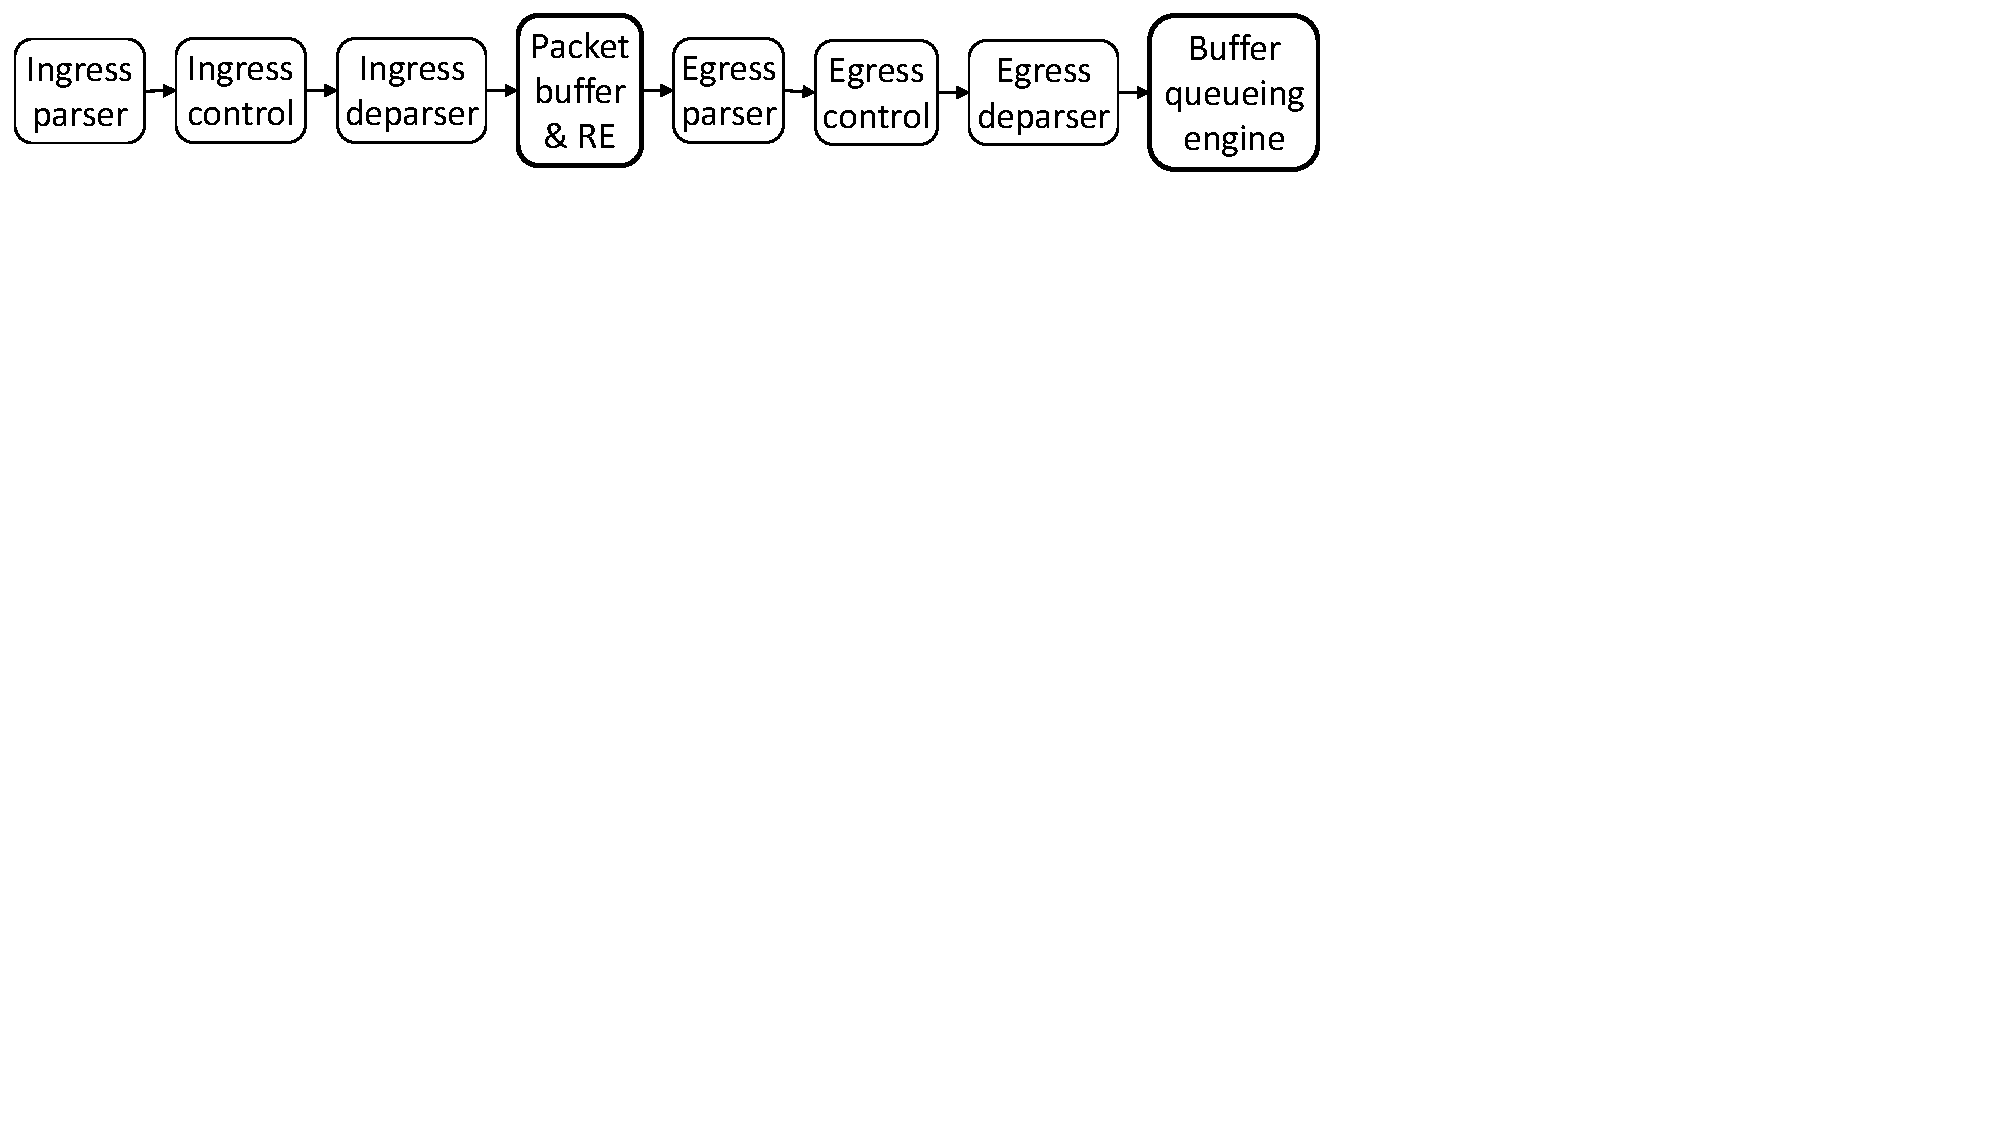
\includegraphics[trim=3 459 281 0, clip,scale=0.35]{psa-pipeline.pdf}
%  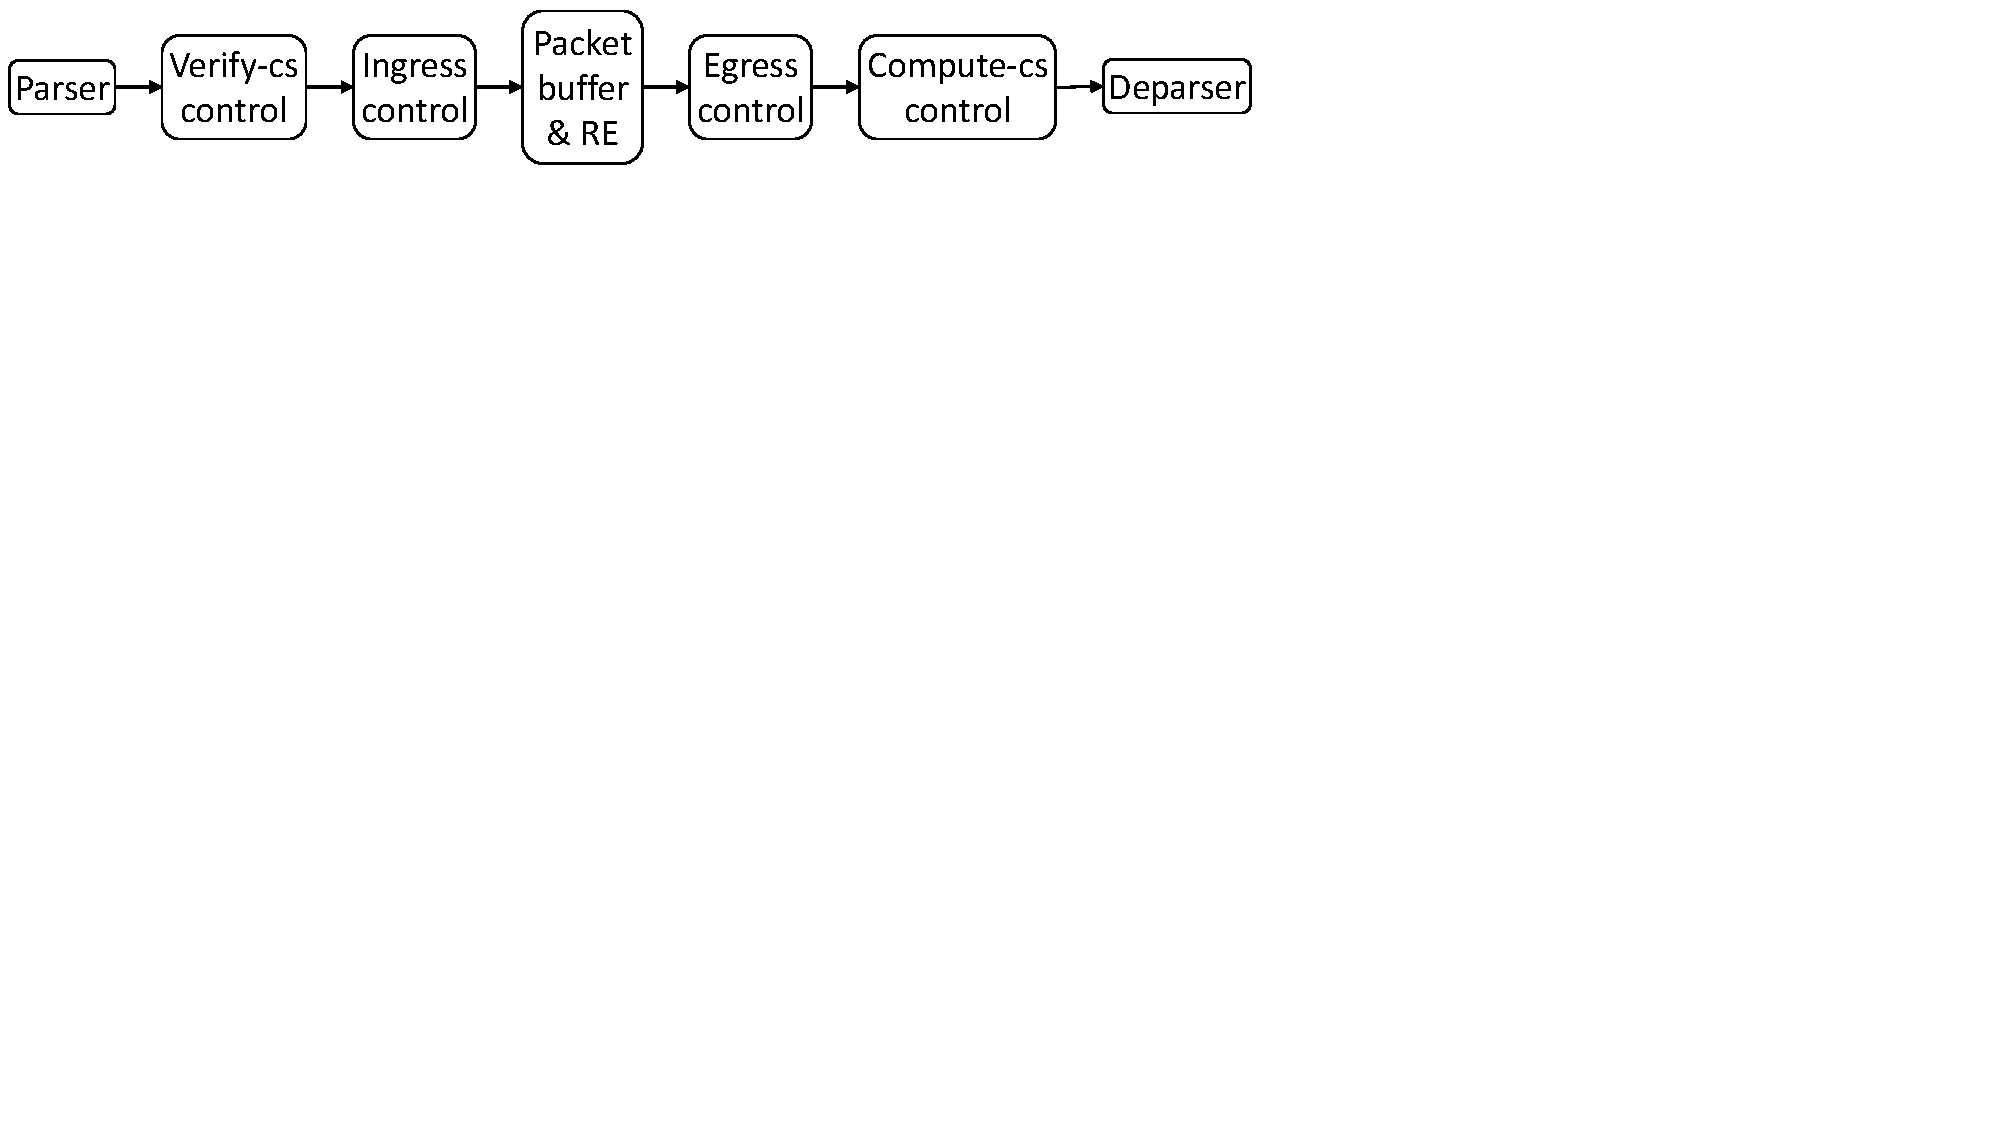
\includegraphics[trim=3 460 357 0, clip,scale=0.35]{v1model-pipeline.pdf}
%  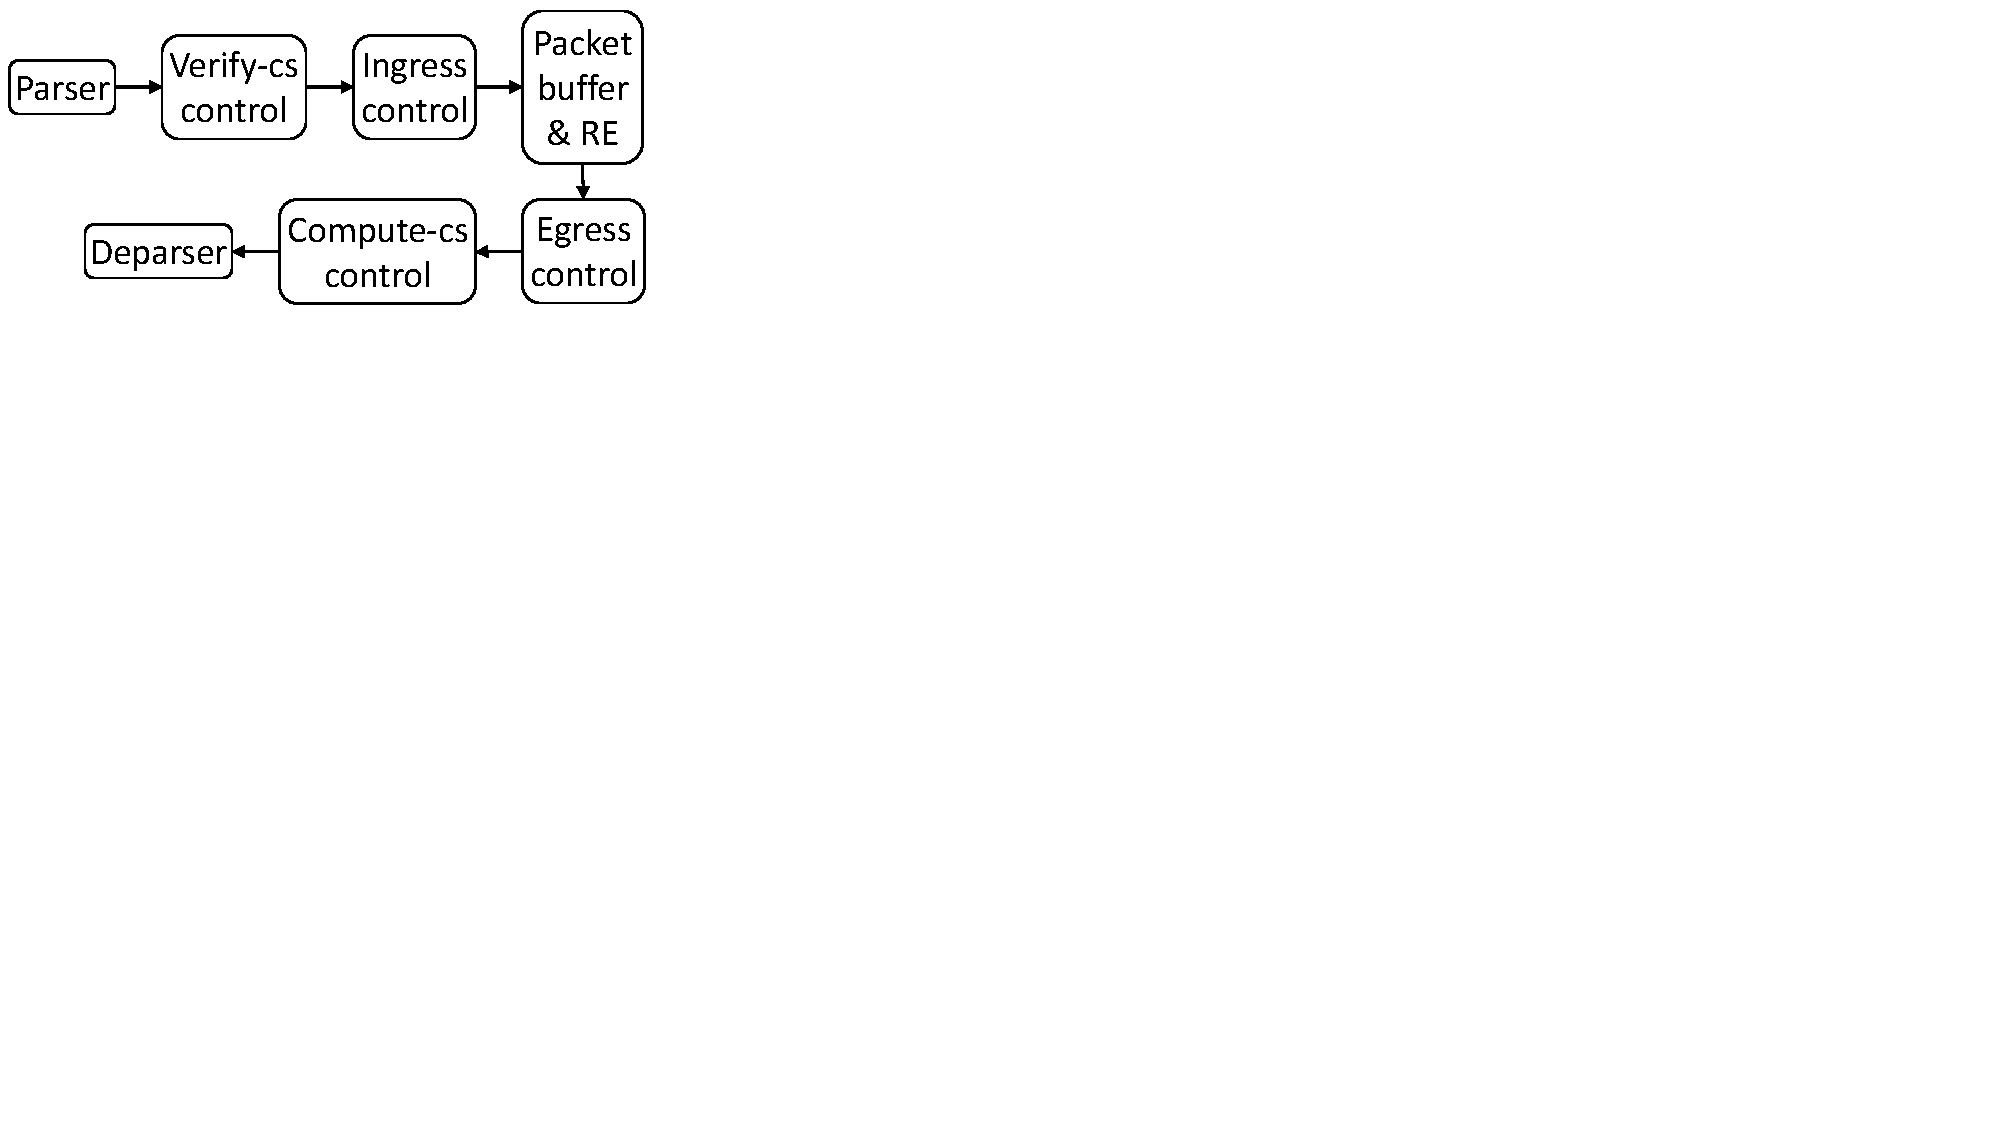
\includegraphics[trim=0 390 650 0, clip,scale=0.5]{v1model-pipeline-wrap.pdf}
%  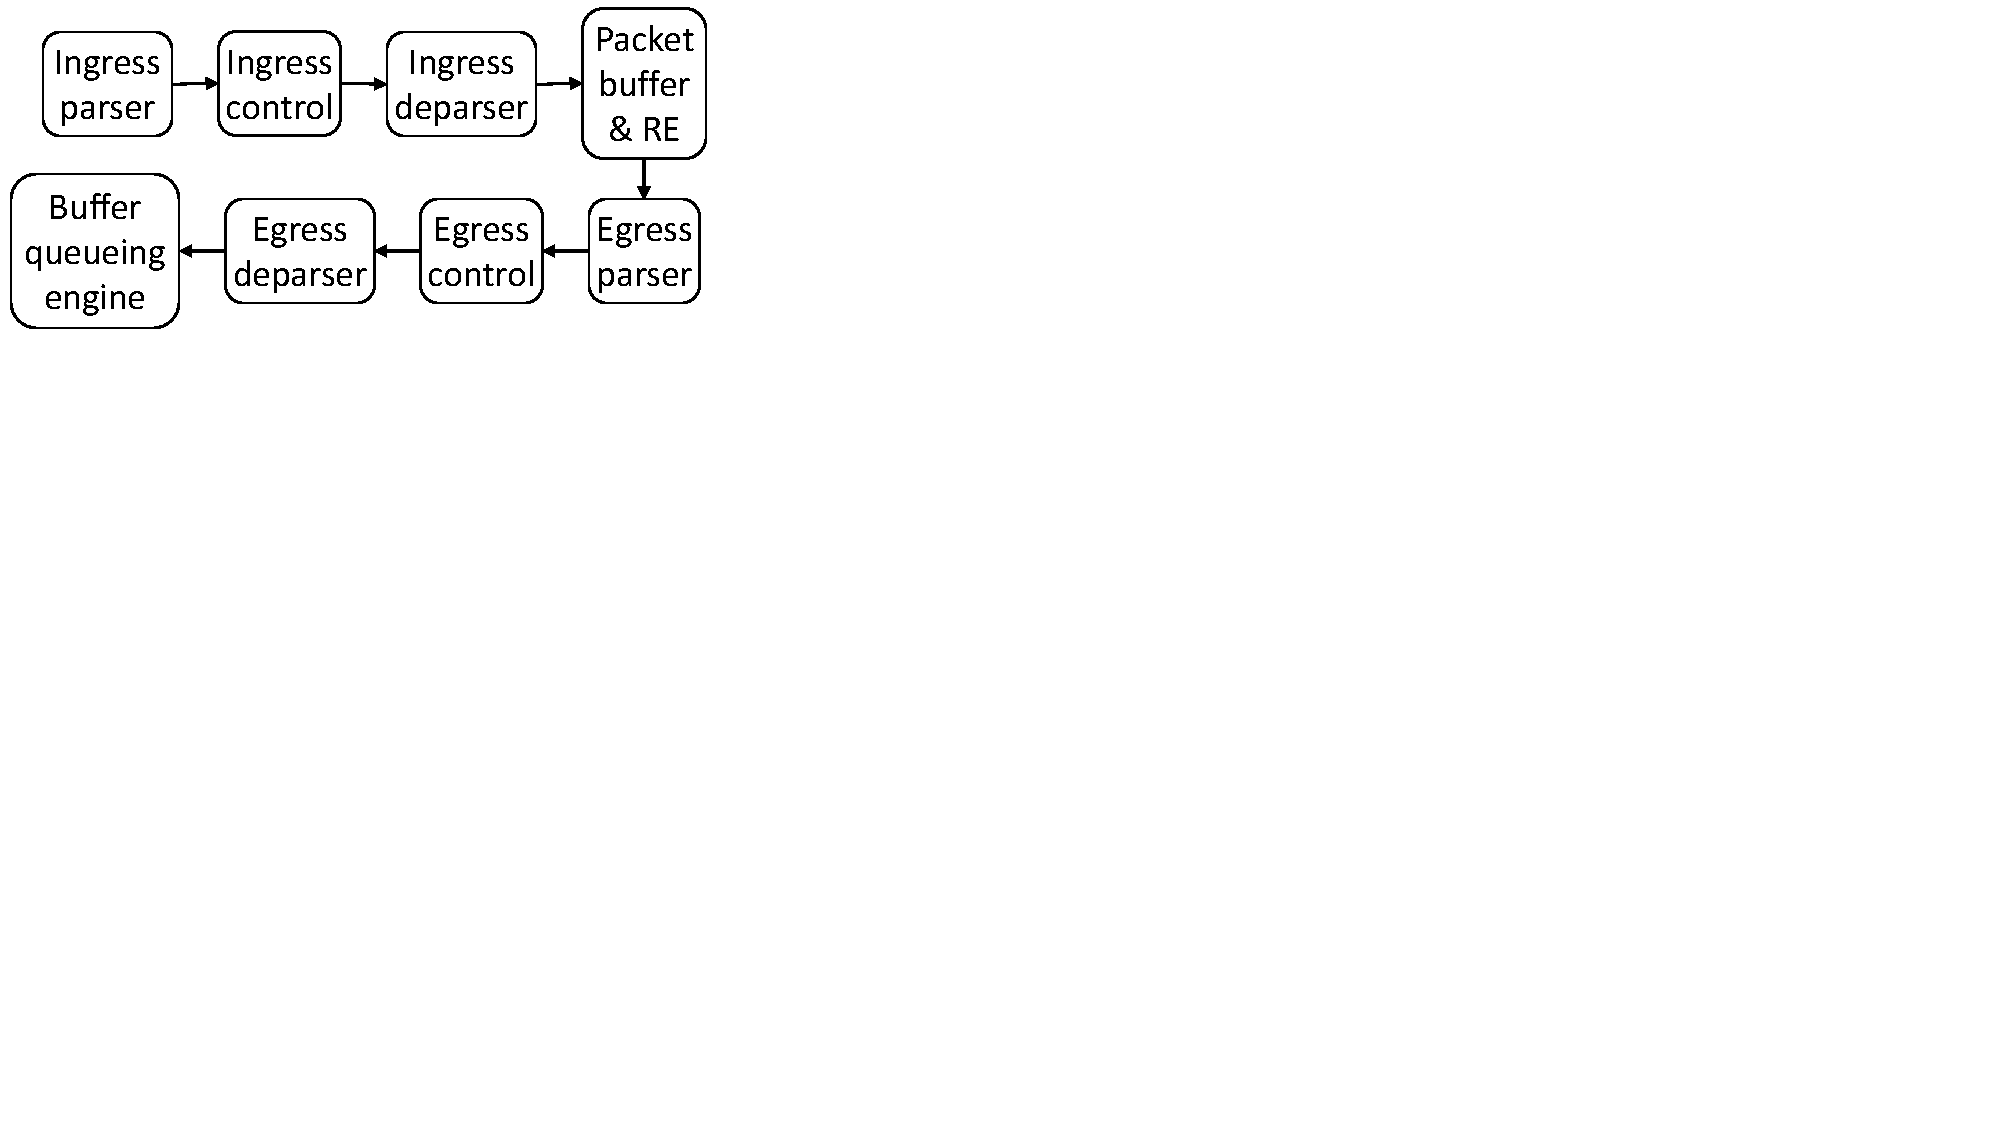
\includegraphics[trim=0 380 620 0, clip,scale=0.5]{psa-pipeline-wrap.pdf}
%  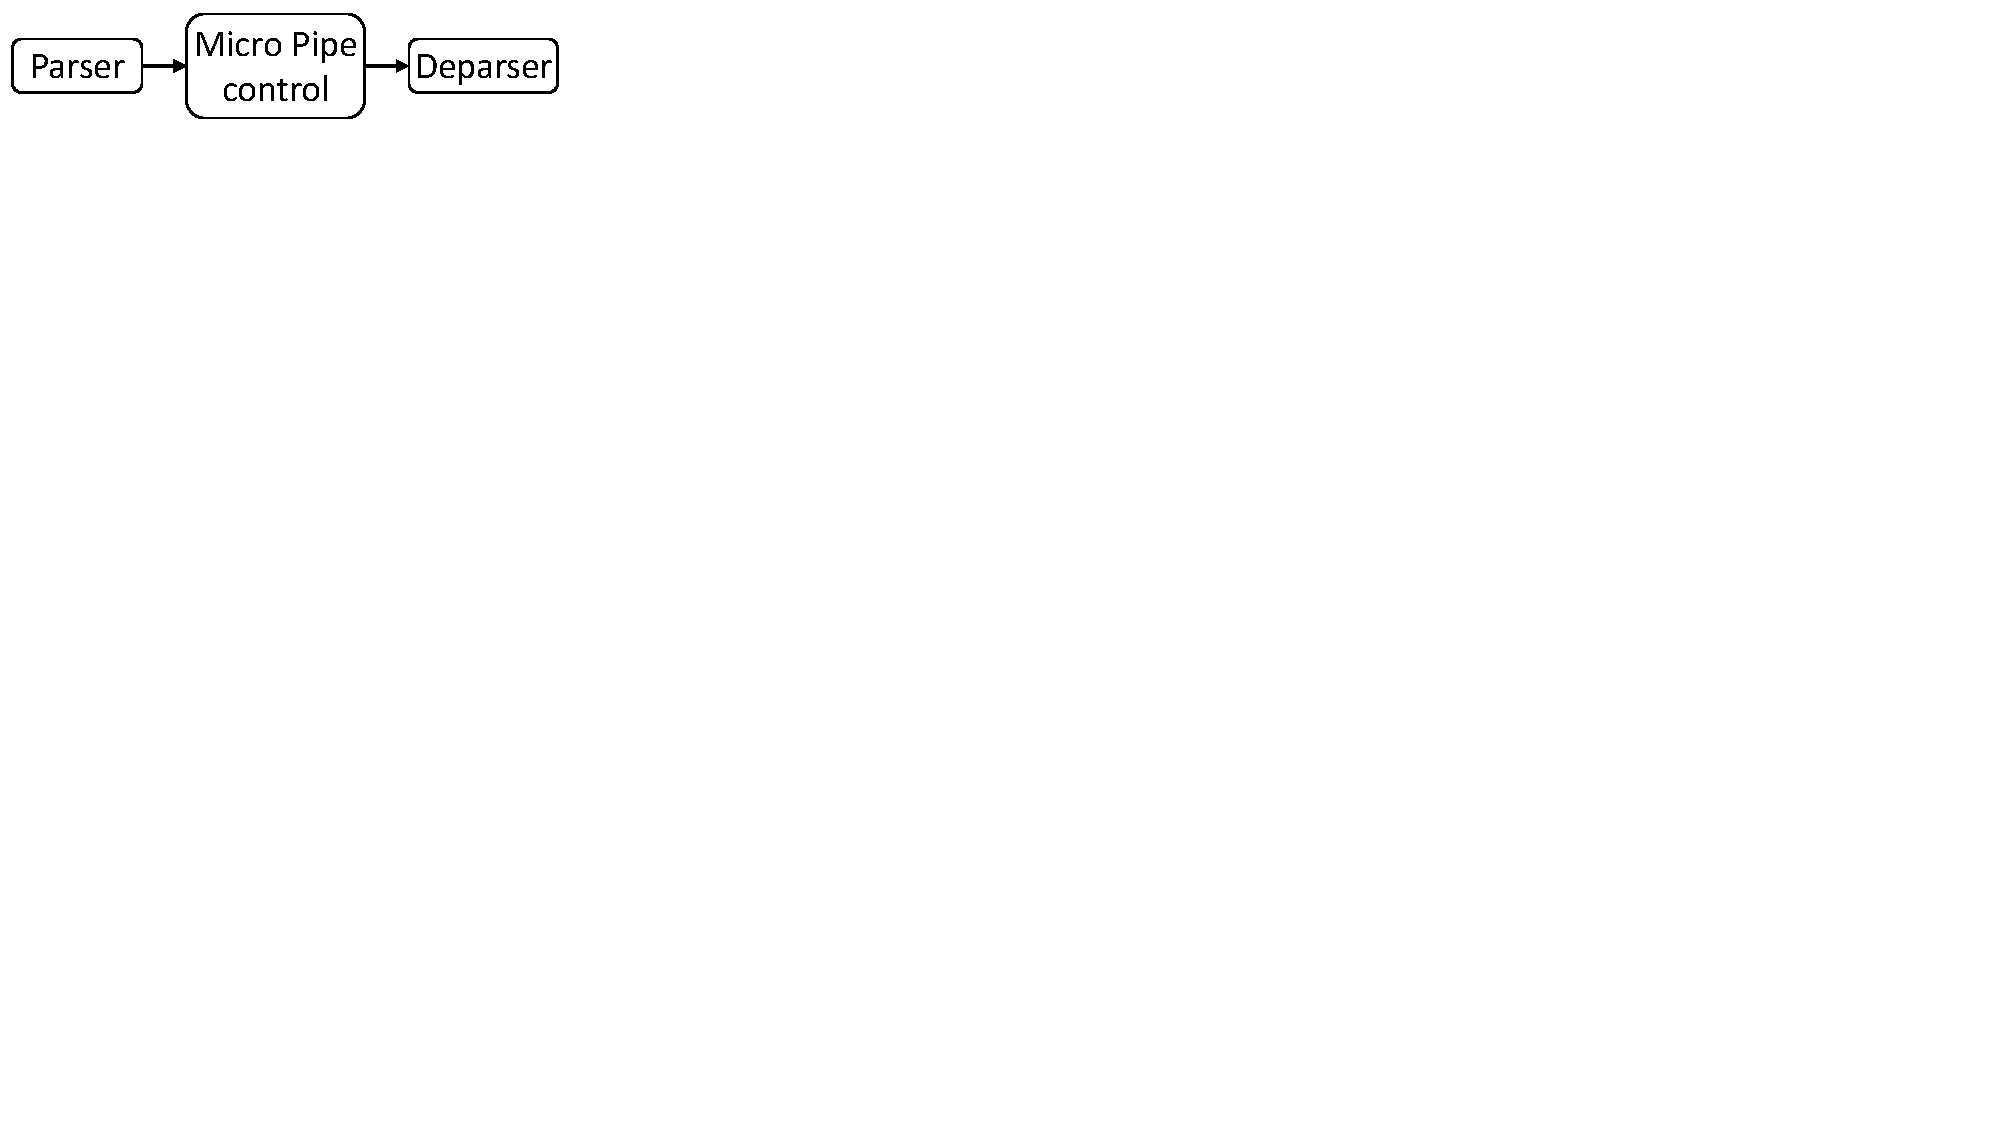
\includegraphics[trim=0 482 692 0, clip,scale=0.7]{msa-pipeline.pdf}
%  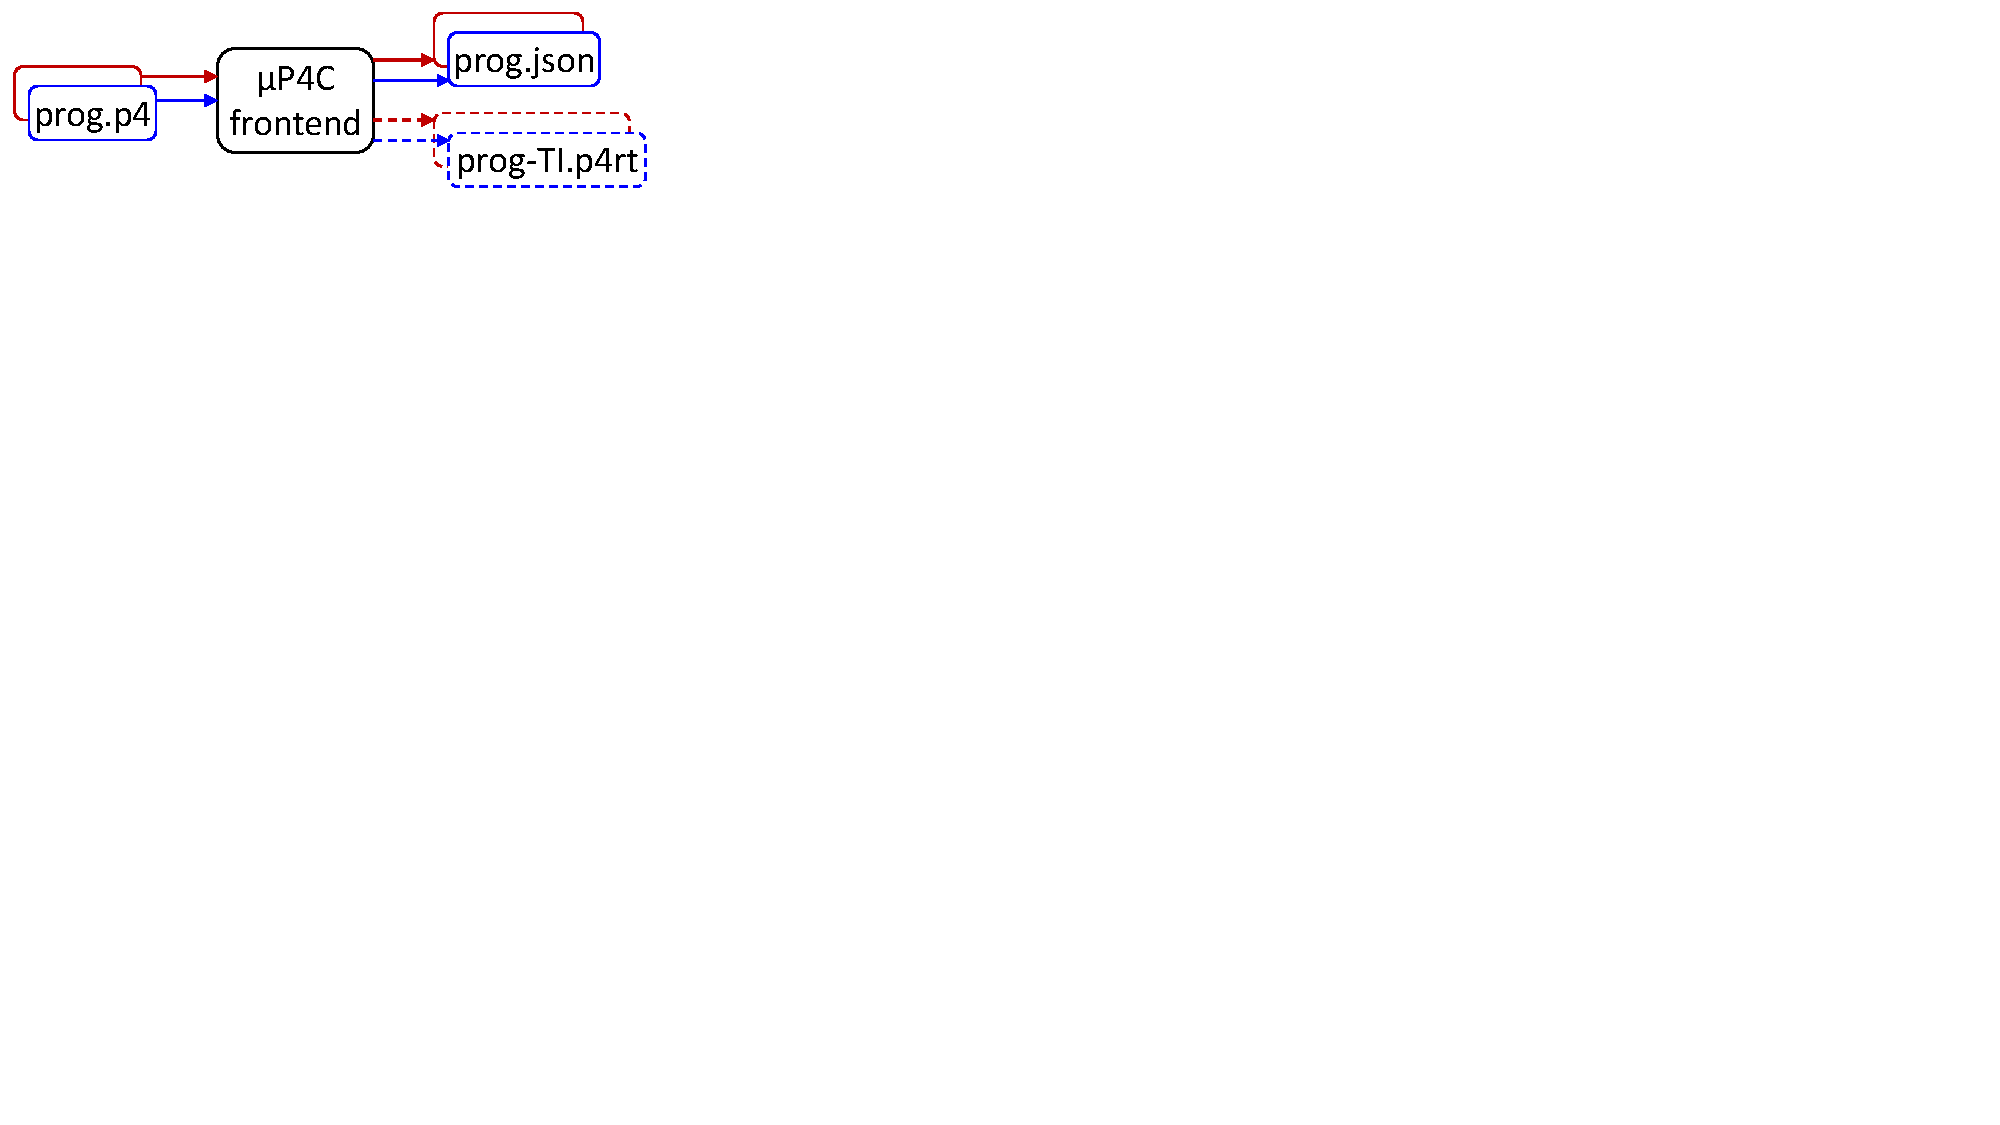
\includegraphics[trim=0 450 645 0, clip,scale=0.6]{mp4c-frontend.pdf}
%  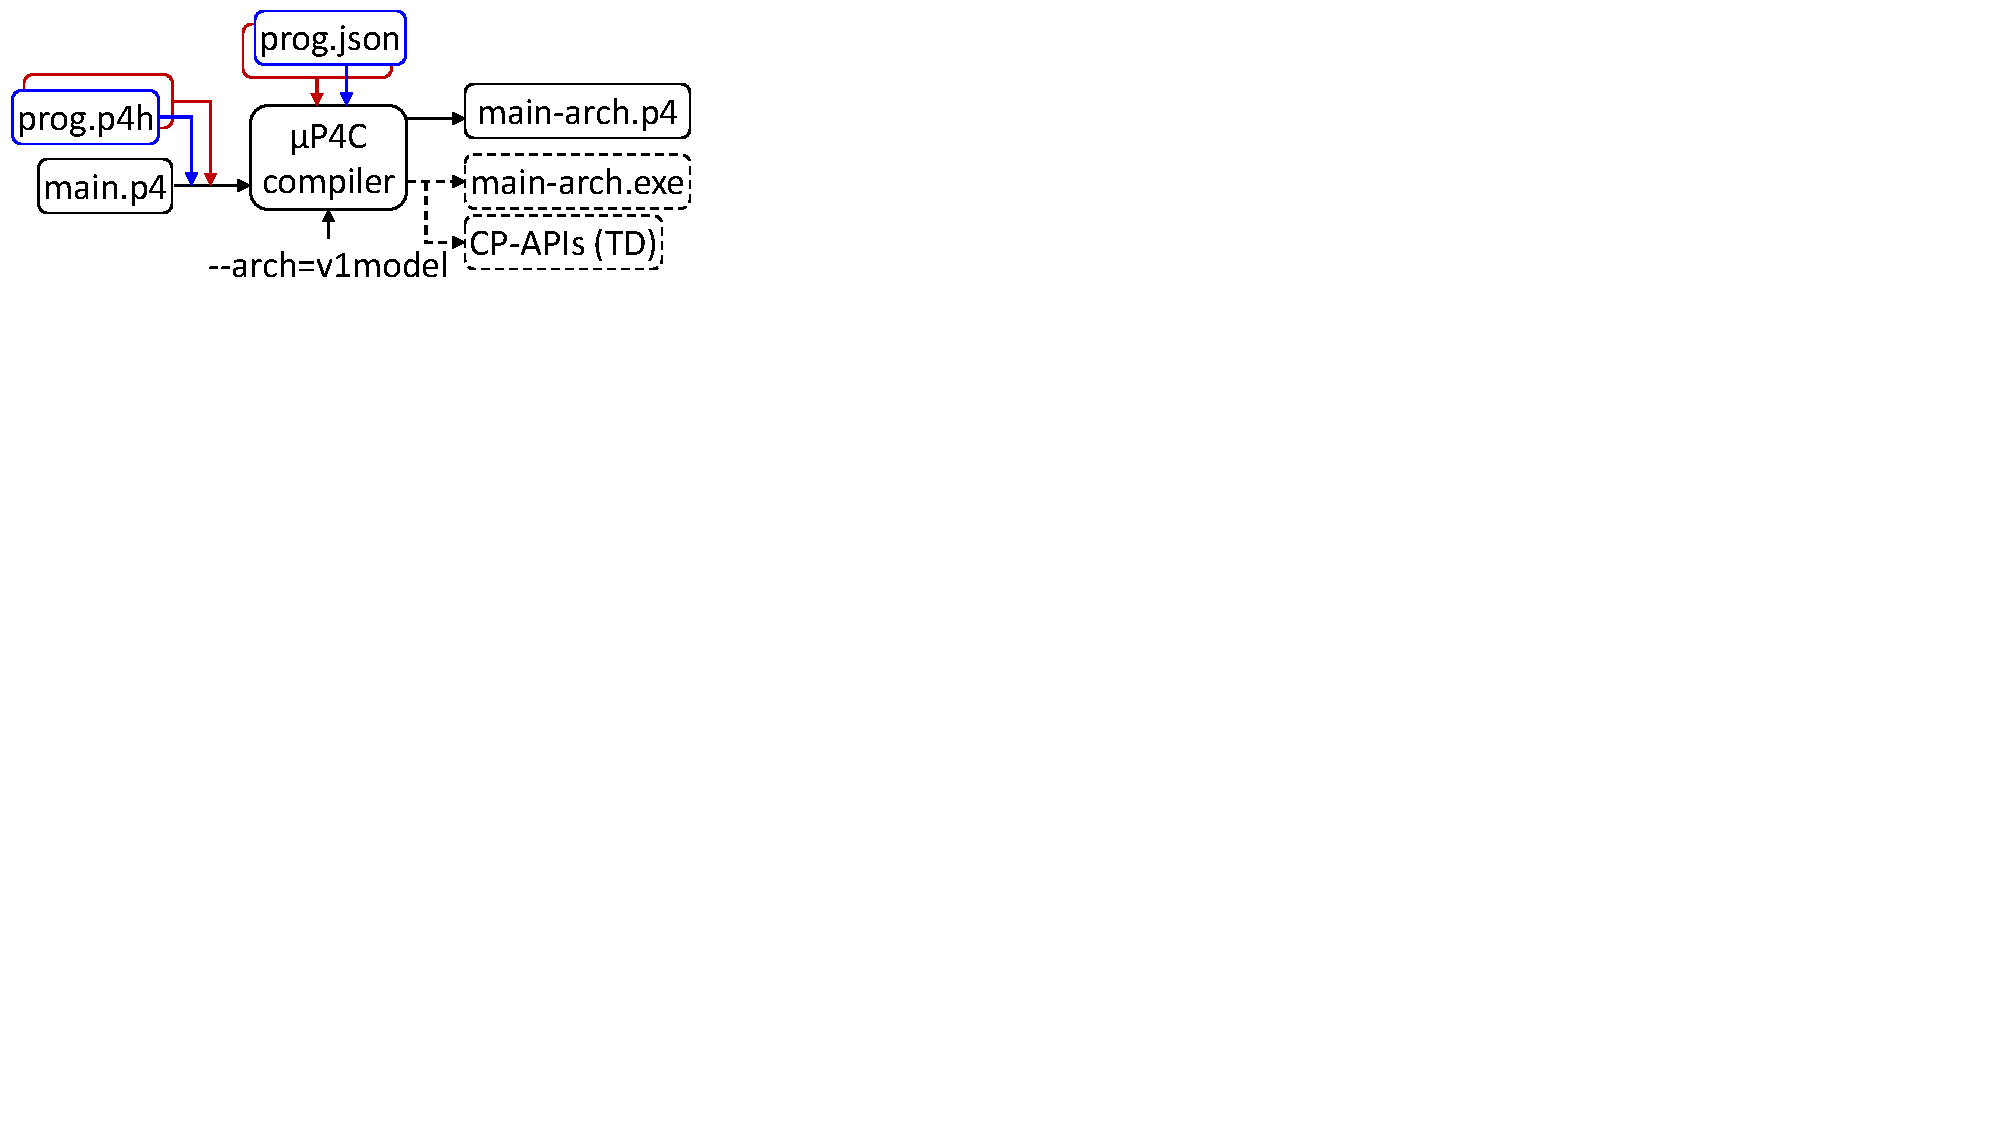
\includegraphics[trim=0 405 623 0, clip,scale=0.7]{mp4c-compiler}
%  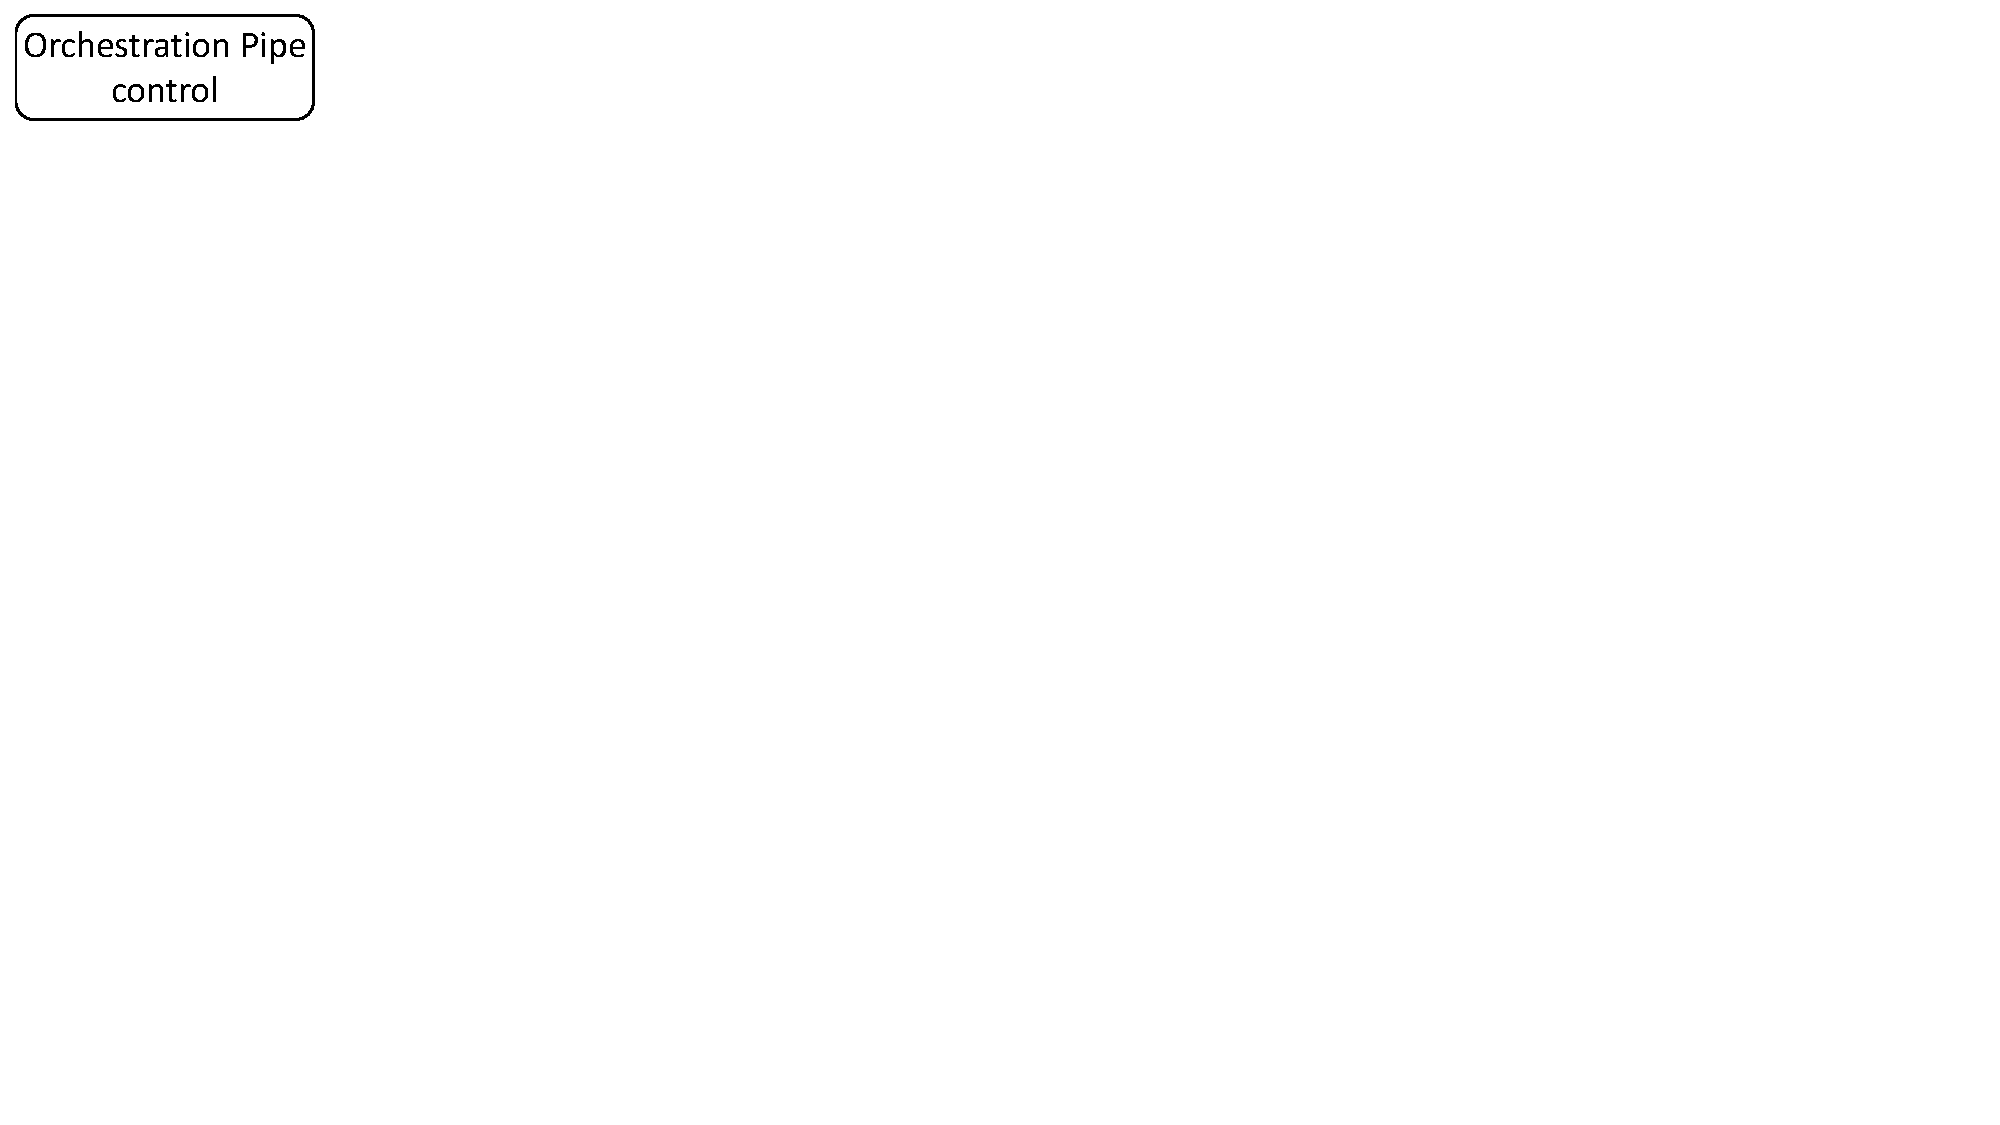
\includegraphics[trim=0 480 805 0,clip,scale=0.5]{micro-orchestration-pipeline}
% \end{figure}


\section{Micros P4}

overview:


Define types of composition: 
Sequential
Parallel


What do we need to provide interface to code modules?

We need runtime behaviour with package. 
packet, sm, es, inargs, inout args -> package -> packet, sm, es, out args, inout args
P4 extended to 
allow Define new Package types
runtime behavior with package types

MicroP4 defines package interfaces.


MicroP4 captures intrinsic metadata dependency of real targets using logical extern (egress\_spec)

MicroP4 defines common abstractions for target specific operations that can not be expressed in P4
e.g., multicast



Micro P4 higher-level description and usage:

% \begin{figure}
%     \begin{subfigure}{0.45\linewidth}
%         \centering
%         \includegraphics{\}
%         \label{subfig:micro}
%     \end{subfigure}
% \caption{Runtime Behavior of Package Types}
% \label{fig:E-msa-pipelines}
% \end{figure}

Architecture model of real targets provides a default path, comprising  processing blocks, for packet and data in data plane pipeline.
Programmers can use target-specific externs to change the default path and route the packet through required processing block.
Intuitively, we can say that the packet-processing code is stationary whereas packet and data are propagated through the stationary code blocks in pipeline.
P4 compiler backends of real targets mandates programmers to map logic and provide code for different processing units in data plane instead of automatically allocating code to the units. 

Micro-Switch Architecture, $\mu$SA, is designed with completely opposite philosophy.
$\mu$SA provides abstraction to avail features of maximum processing blocks at any stage of execution-control of a program and $\mu$P4C compiler transforms code according to the abstractions to allocate on stationary processing blocks of the real target device.

\begin{figure}[!h]
    \begin{subfigure}{\linewidth}
        \centering
        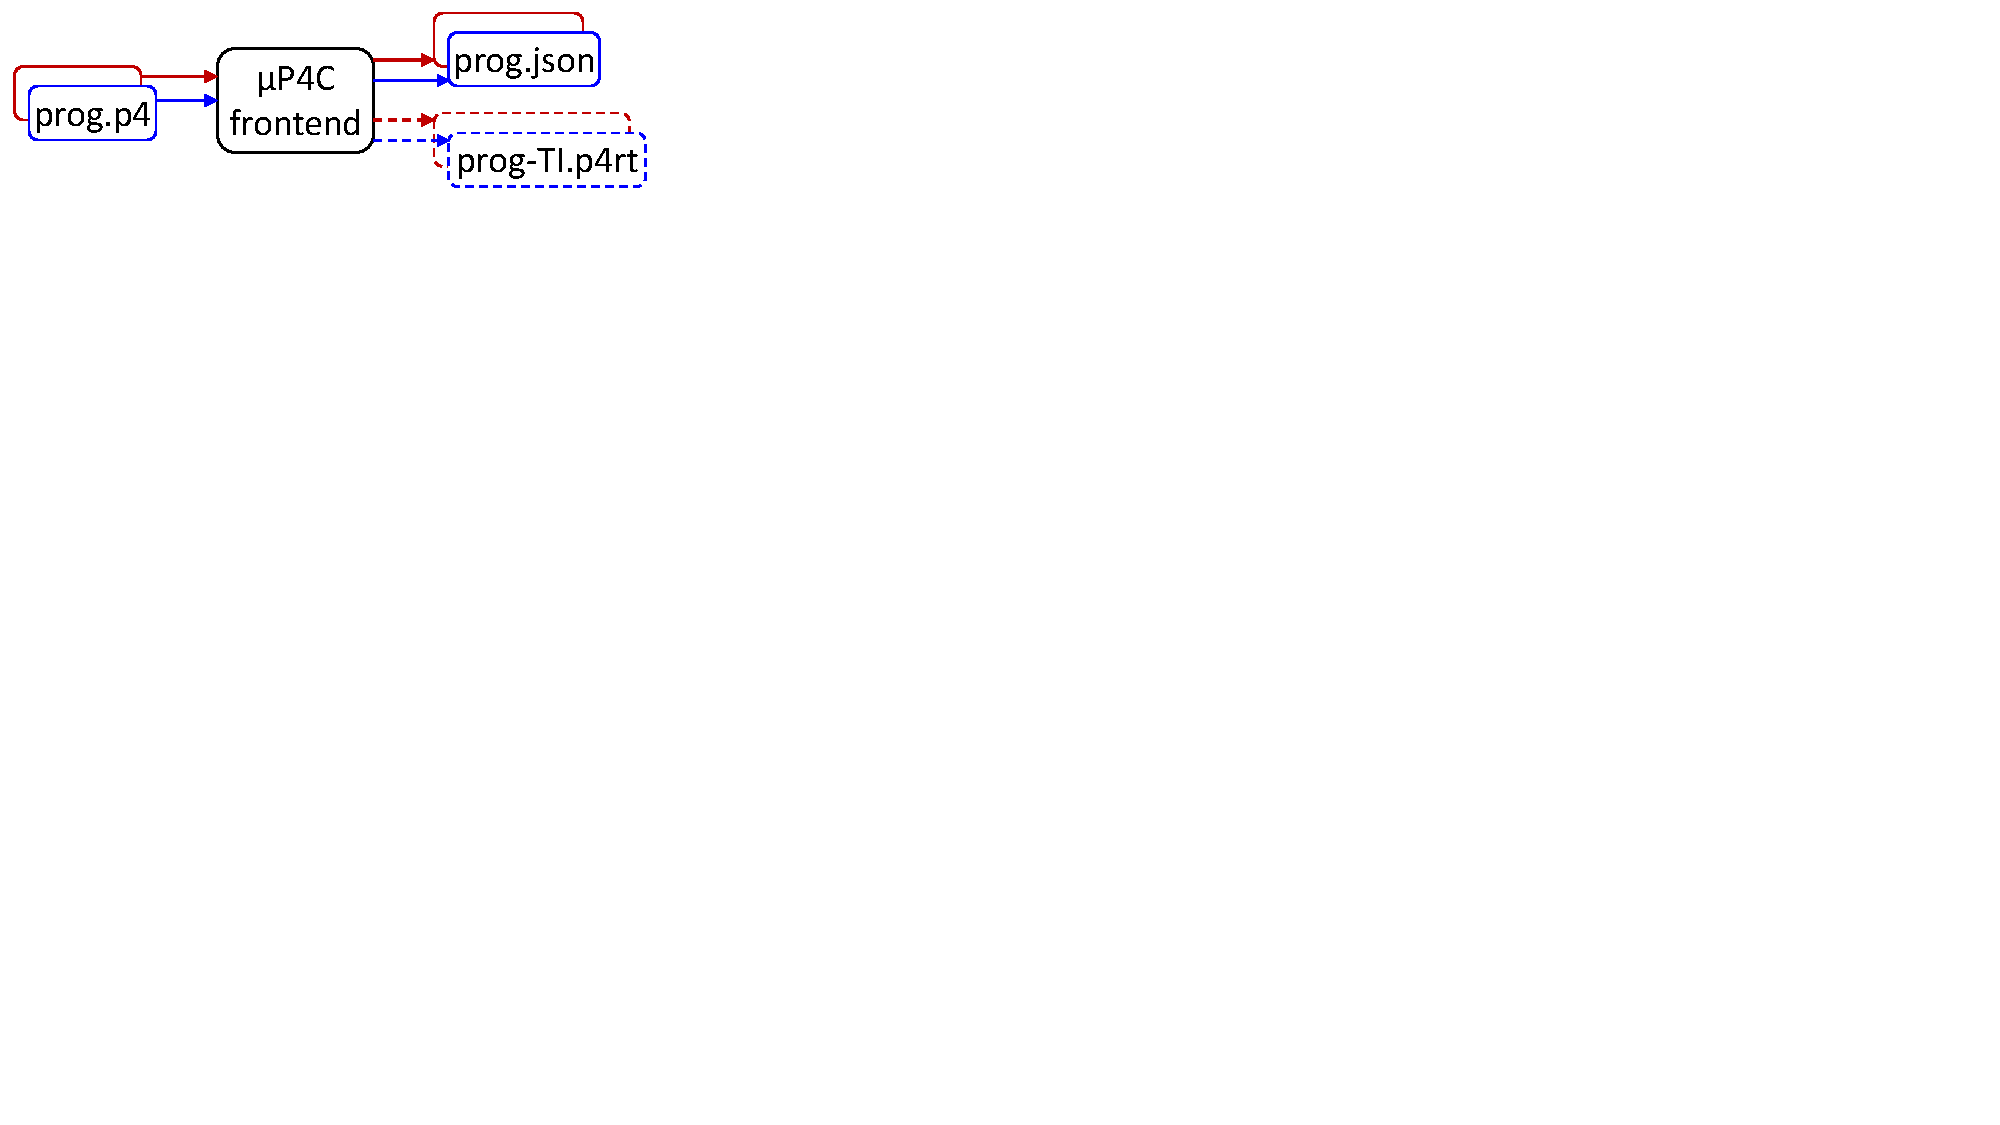
\includegraphics[trim=0 450 645 0, clip,scale=0.55]{mp4c-frontend}
        \caption{Library Program Compilation}
        \label{subfig:compiling-modules}
    \end{subfigure}
    \begin{subfigure}{\linewidth}
        \centering
        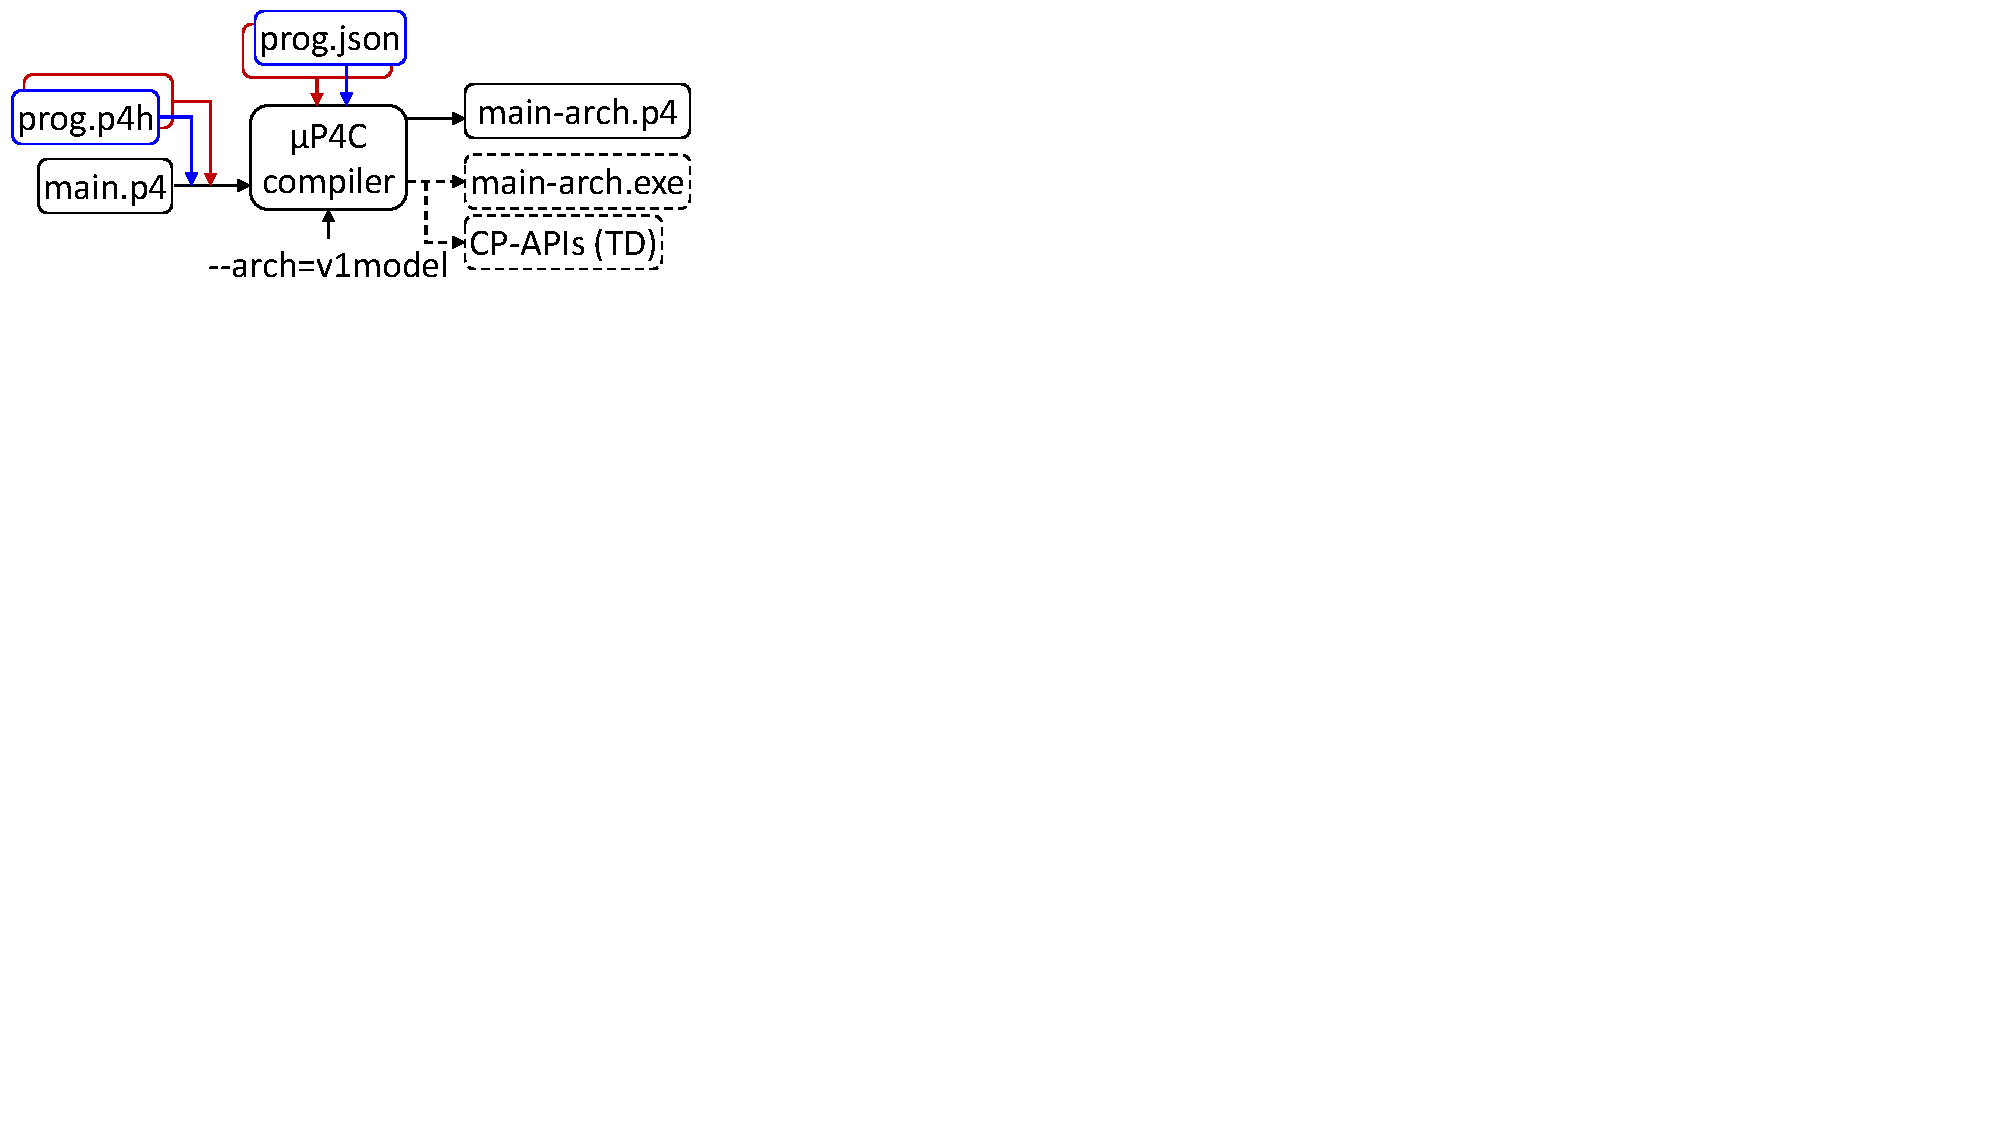
\includegraphics[trim=0 405 623 0, clip,scale=0.55]{mp4c-compiler}
        \caption{Composition and Translation of Main Instance}
        \label{subfig:composition-translation-of-main-instance}
    \end{subfigure}
\caption{Compiling $\mu$SA programs}
\label{fig:compiling-msa-programs}
\end{figure}



\section{Micros-Switch Architecture}
\label{section:micros-awitch-architecture}
$\mu$SA, is designed for a logical target, unlike fixed pipeline of real target data planes with stationary processing blocks.
$\mu$SA provides multiple types of logical pipelines.
For each pipeline type, it exposes an interface type comprising a set of programmable blocks.
Programmers can define a P4 \texttt{package} type by implementing all the programmable blocks of a interface type.
In the same source file, programmers can provide multiple implementations of the same interface type to define multiple package types.
$\mu$SA pipelines do not have fixed-function blocks, instead it provides a set of logical externs which can be instantiated and used within control blocks of the $\mu$SA pipelines.
This design choice reduces heterogeneity in abstract model of data plane programs.

$\mu$SA defines various architecture specific structures and externs that allow programmers to express sequential and parallel composition of fine-grained packet processing functions.
It defines standard intrinsic metadata as~\texttt{msa\_sm\_t} as a struct type.
The fields of this struct provide basic information populated by the target e.g.,~\texttt{packet\_length}.
Some fields are not mutable, however $\mu$SA allows to declare instances of the struct and perform assignment operation between two instances to create copies.
Sections~\ref{subsection:pipelines} and~\ref{subsection:logical-externs} describe pipelines and logical externs, respectively.



\subsection{Pipelines}
\label{subsection:pipelines}
$\mu$SA has two types pipeline, Micro and Orchestration.
Figure~\ref{fig:msa-pipelines} shows programmable blocks of two types.
Micro pipeline interface comprises of parser, Micro-Pipe control and Deparser programmable blocks.
Every incoming packet is parsed and validated by the parser, if parser terminates in~\texttt{accept} parse state, then execution-control is transferred to micro-pipe control block.
Depending on use of logical externs in implementation, packet may not complete the processing of the control block.
If the execution-control reaches till the end of the control block, packet is processed by the deparser block.
\begin{figure}[!ht]
    \begin{subfigure}{0.45\linewidth}
        \centering
        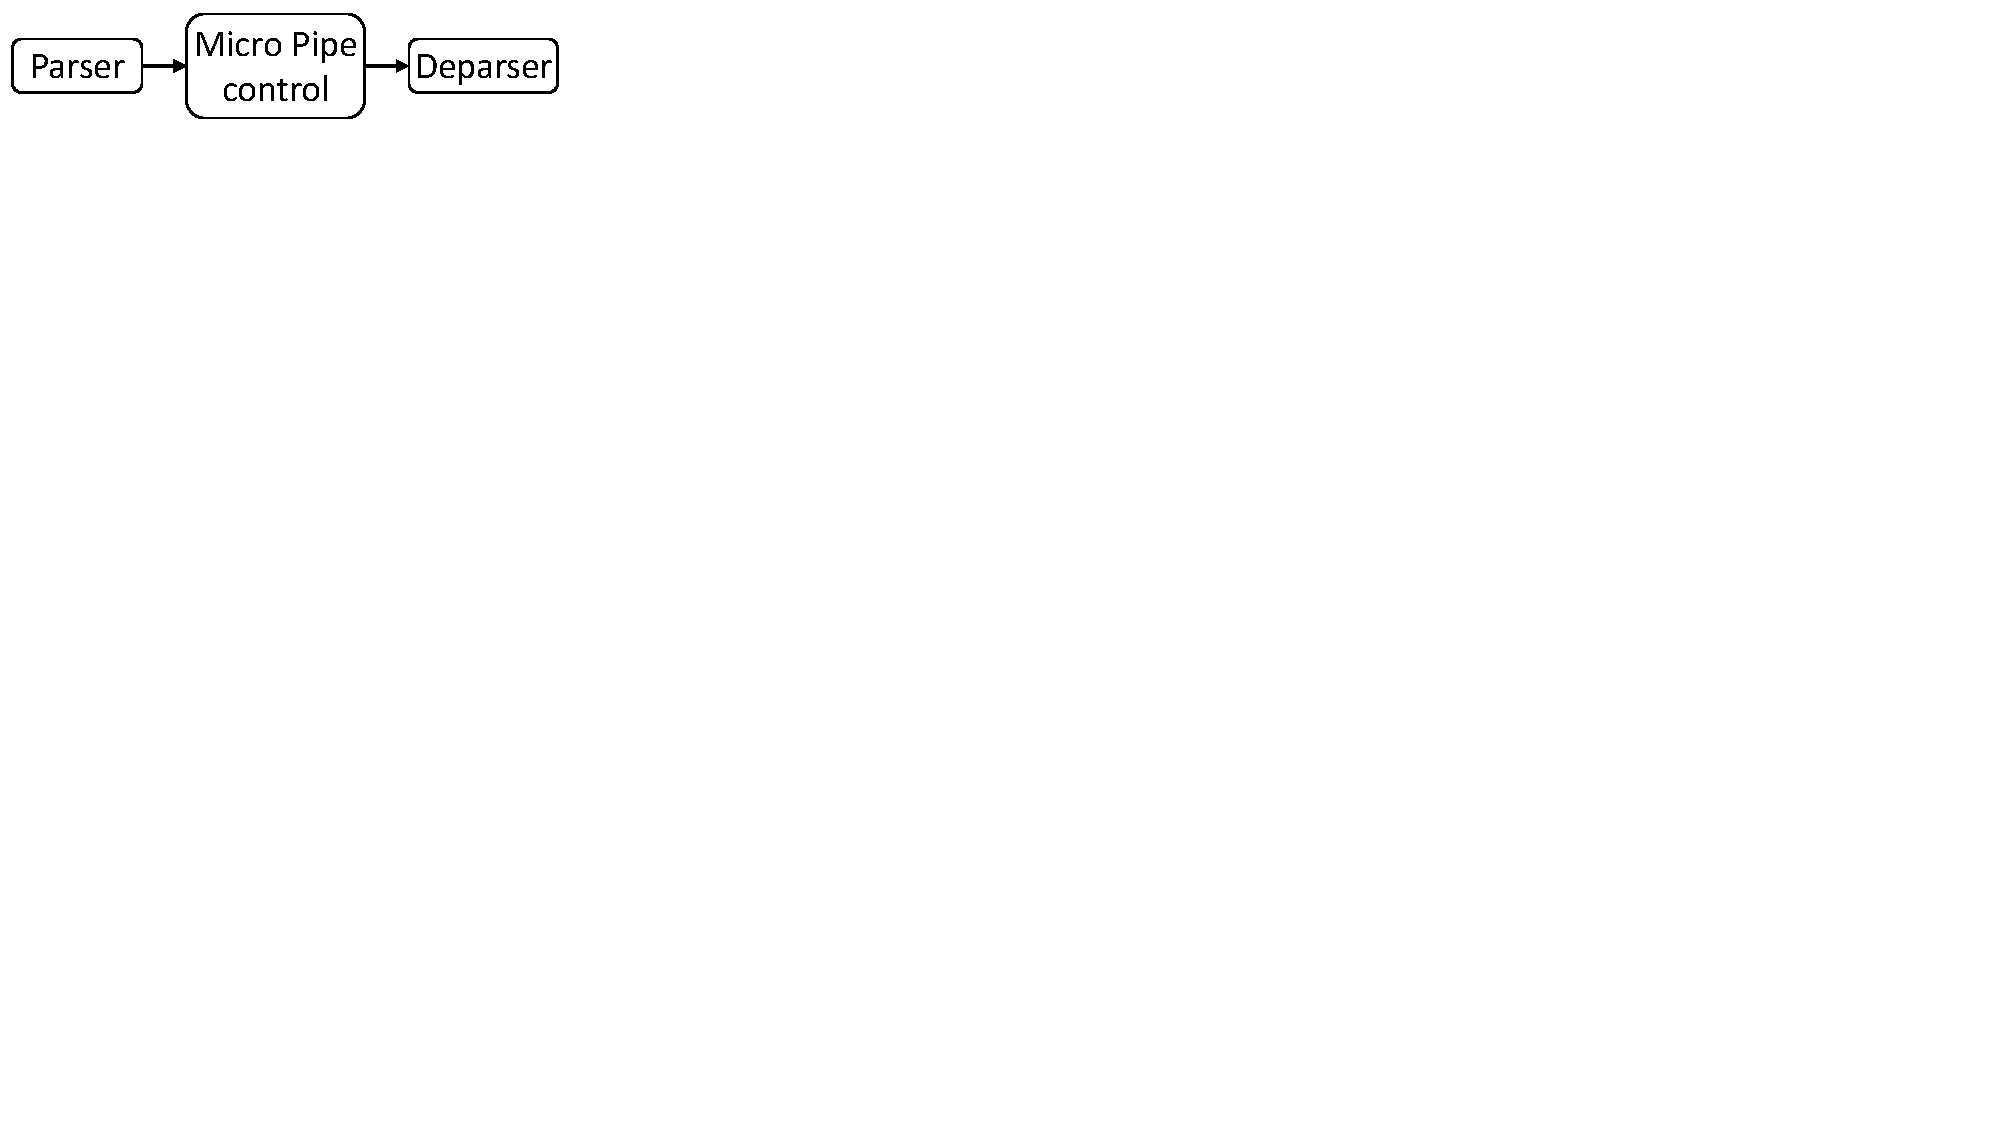
\includegraphics[trim=0 482 692 0, clip,scale=0.45]{msa-pipeline}
        \caption{Micro}
        \label{subfig:micro}
    \end{subfigure}
    \begin{subfigure}{0.45\linewidth}
        \centering
        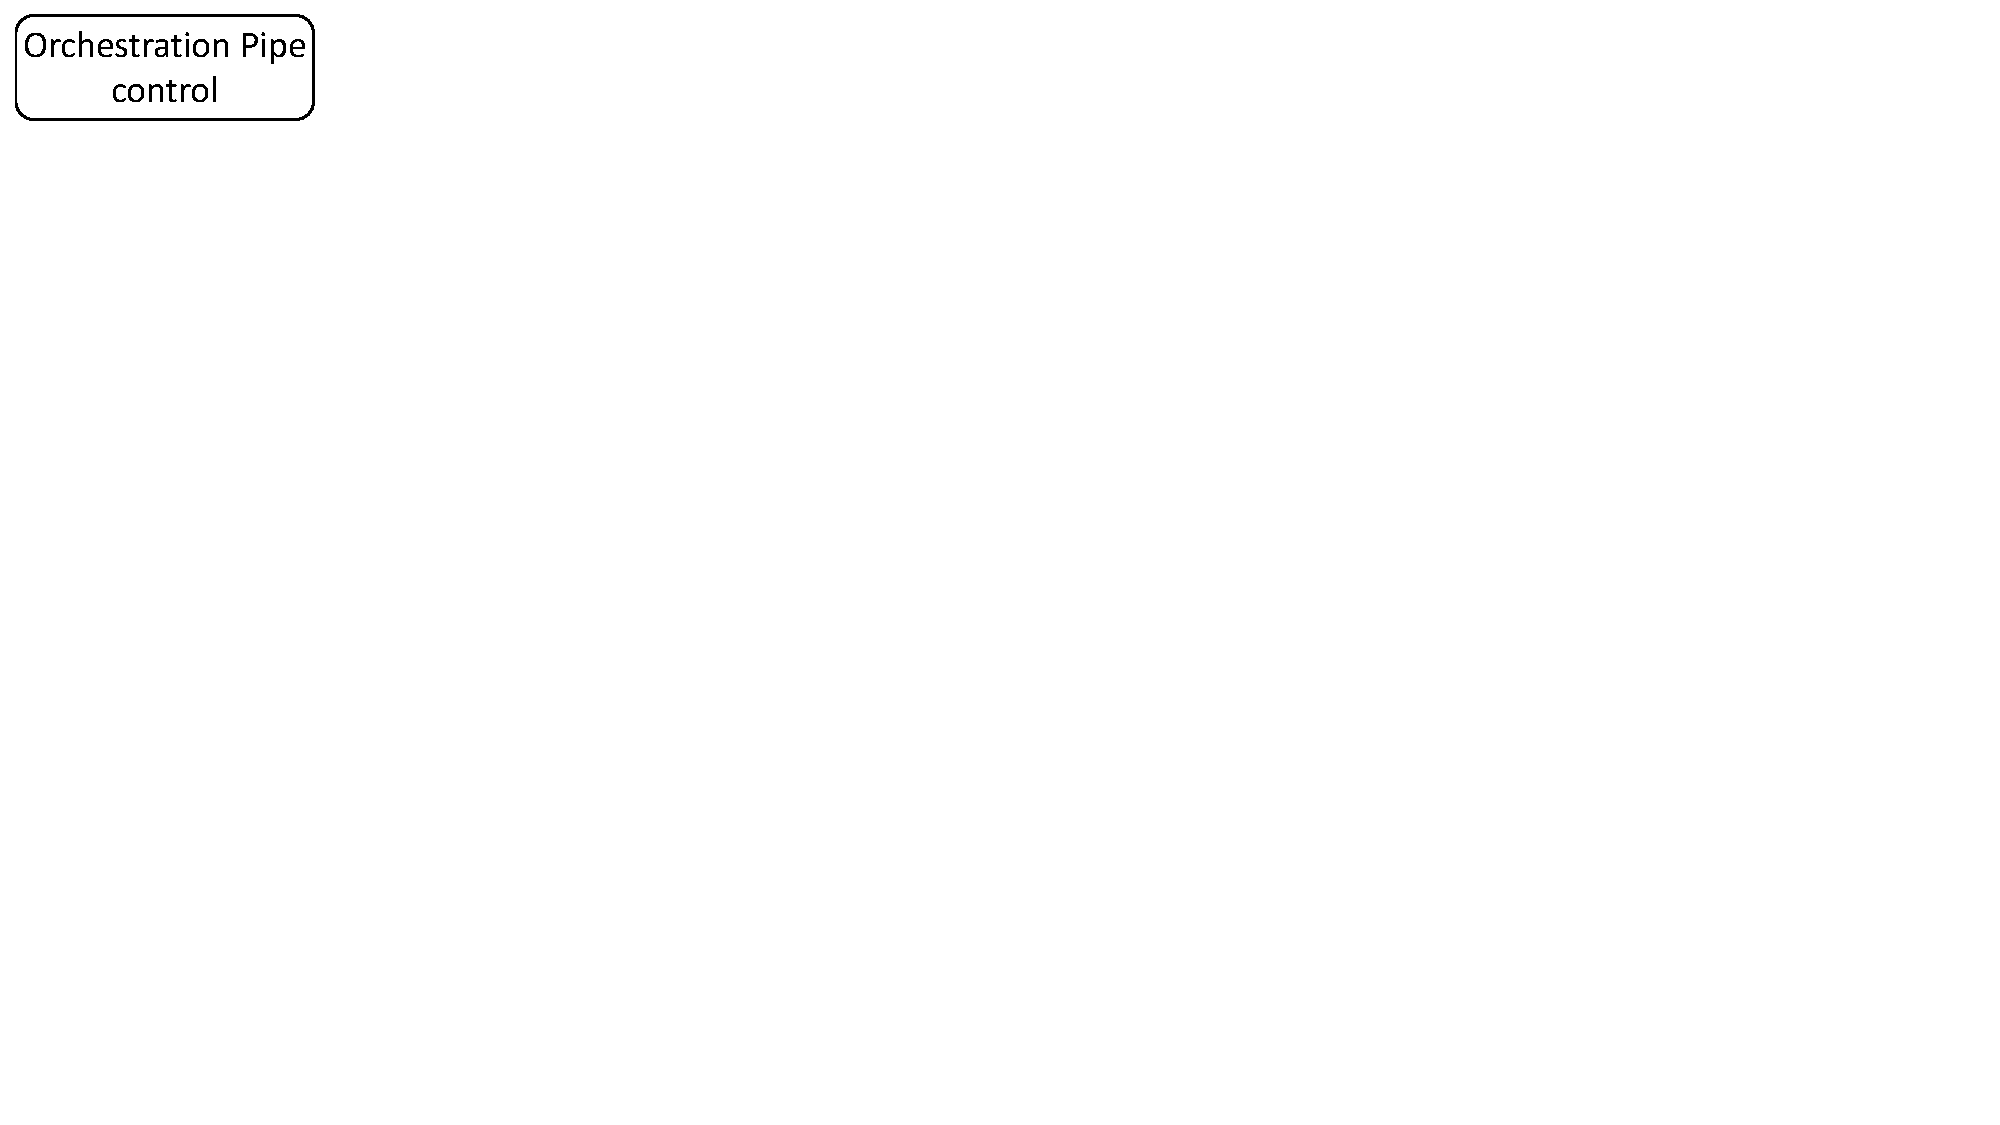
\includegraphics[trim=0 480 805 0,clip,scale=0.45]{micro-orchestration-pipeline}
        \caption{Orchestration}
        \label{subfig:orchestration}
    \end{subfigure}
\caption{$\mu$SA Pipelines}
\label{fig:msa-pipelines}
\end{figure}

Orchestration pipeline interface has only a control block, orchestration pipe.
Programmers can implement imperative control flow using intrinsic metadata of $\mu$SA and runtime parameters to the package types.
In addition of existing language features, it allows programmers to instantiate package types and invoke them in the body(~\texttt{apply}) of the control block.



% \begin{figure*}
% \noindent \begin{minipage}[t]{\linewidth}
% \begin{lstlisting}[frame=none]
% 
% Orchestration<I, O, IO, U, R>(msa_packet_in b, msa_packet_out po, inout msa_sm_t sm, egress_spec es, in I iargs, out O oargs, inout IO ioargs) ()
% 
% MicroSwitch<I, O, IO, U, R>(msa_packet_in b, msa_packet_out po, inout msa_sm_t sm, egress_spec es, in I iargs, out O oargs, inout IO ioargs) ()
% 
% \end{lstlisting}
% \end{minipage}
% \vspace*{-10pt}
% \caption{$\mu$SA Pipeline Interface Types}
% \end{figure*}


\subsection{Logical Externs}
\label{subsection:logical-externs}

TODO rename ``function'' to ``mehod''.
\subsubsection{Packet Externs}
Packets are represented using \texttt{packet\-\_in} and \texttt{packet\_out} externs defined in P4-16 core library~\cite{core.p4}.
However, these externs do not provide functions and semantics required to describe sequential and parallel composition of programs.
We define $\mu$SA specific packet externs to allow programmers to express sequential and parallel processing. 
$\mu$SA specific packet externs \texttt{msa\_packet\_in} and \texttt{msa\_packet\_out} contain an instance of \texttt{packet\_in} and \texttt{packet\_out}, respectively.
We introduce a function, \texttt{get\-\_packet\-\_in}, in \texttt{msa\-\_packet\-\_out}.
\begin{lstlisting}[frame=none]
void get_packet_in(msa_packet_in msa_pin);
\end{lstlisting}
Similarly, we introduce copy\_from function in \texttt{msa\_packet\_in} that replicates the state of passed argument (\texttt{msa\_pin}) to the calling instance.
\begin{lstlisting}[frame=none]
void copy_from(msa_packet_in msa_pin);
\end{lstlisting}
\subsubsection{Egress Specifications}
To support special features, the architectures of real target devices provide intrinsic metadata  that depends on operations on other intrinsic metadata.
For example,  many real targets allow to measure every packet's queuing latency through the device.
The queuing latency is computed by recording enqueue and dequeue timestamps in the device.
These timestamps can be measured only after the packet's egress port is finalized and the packet is sent to the packet buffer.
The architectures of real target devices expose timestamps as intrinsic metadata which can be accessed only after the egress port is finalized.
\begin{figure}[!h]
\begin{lstlisting}[frame=none]
enum msa_metadata_t {
  INGRESS_TIMESTAMP,
  EGRESS_TIMESTAMP
}
extern egress_spec {
  void set_egress_port(in bit<8> port);
  bit<8> get_egress_port();
  bit<32> get_value(in msa_metadata_t ft);
  void copy_from(egress_spec es);
}
\end{lstlisting}
\caption{Egress\_Spec Extern}
\label{fig:msa-egress-spec-extern}
\end{figure}
$\mu$SA considers \texttt{egress\_spec} as a stateful extern object (Figure~\ref{fig:msa-egress-spec-extern}) providing functions to set and get \texttt{egress\_port} and retrieve values of other egress\_port dependent intrinsic metadata.
$\mu$P4C allows repeated usage of the extern's functions in the single control block of $\mu$SA pipelines.
$\mu$P4C uses their occurrences to transform the code to multi-control pipelines of real target architectures.
If \texttt{get\_value} occurs before \texttt{set\_egress\_port} on any possible execution-control path, $\mu$P4C raises a compile-time error.

\subsubsection{Packet Buffer}
$\mu$P4 allows programmer to express parallel processing of multiple P4 programs by passing the copy of the packet and intrinsic metadata to multiple programs.
Programmers can use assignment statements to create copies of standard intrinsic metadata (msa\_sm\_t) and use~\texttt{copy\_from} functions in~\texttt{msa\_packet\_in} and~\texttt{egress\_spec} to create copies of the packet and intrinsic metadata.
In addition, it provides logical a packet buffer as an extern (Figure~\ref{fig:msa-packet-buffer-extern}) to serialize output packet and intrinsic metadata.
The logical buffer extern can only be instantiated in the control block of orchestration pipeline.
Its functions can be used only in apply body of the control block.
The output of the multiple programs generated by processing the same packet can be enqueued in the logical buffer.
The dequeue function allows to fetch the packets and either pass it to another program to process or assign it to the msa\_packet\_out argument of orchestration pipe control block.
\begin{figure}[!h]
\begin{lstlisting}[frame=none]
extern msa_packet_buffer<ET> {
  msa_packet_buffer();
  void enqueue(msa_packet_out po, in msa_sm_t sm, egress_spec es, in ET data);
  void dequeue(msa_packet_in pin, out msa_sm_t sm, egress_spec es, out ET data); 
}
\end{lstlisting}
\caption{Packet Buffer Extern}
\label{fig:msa-packet-buffer-extern}
\end{figure}
\subsubsection{Multicast Extern}
$\mu$SA's multicast extern (Figure~\ref{fig:msa-multicast-extern}) can be instantiated in the control blocks of its pipelines.
The \texttt{set\_multicast\_group} can be used to assign replication group to the packet. 
The \texttt{apply} function is allowed to use only in \texttt{apply} body control blocks. 
It is analogous to~\texttt{fork} system call in C except that processing of original packet terminates at the apply call.
It returns instance id of the replicated packets and populates the egress\_spec instance with the port id set by the control plane.
$\mu$P4C translates this extern to multicast mechanism defined in architectures of real targets.
We assume these architectures would have sufficient fields to program their replication engine, so that a combination of the fields can be used as packet instance id.
\begin{figure}[!h]
\begin{lstlisting}[frame=none]
extern msa_multicast_engine {
  msa_multicast_engine();
  void set_multicast_group(GroupId_t gid);
  PacketInstanceId_t apply(egress_spec es);
}
\end{lstlisting}
\caption{Multicast Extern}
\label{fig:msa-multicast-extern}
\end{figure}

\section{$\mu$P4C Compiler}
\label{section-mp4c-compiler}
$\mu$P4 


\subsection{Parser Block Transformation}
\label{subsection:parser-block-transformation}
P4 parser blocks describe parse graphs as state machines.
Real target devices contain programmable parser module that can be programmed using parse graphs.
From the design of programmable parser~\cite{6665172}, we make following observations.
Programmable parsers are implemented using buffer, state machine logic, Ternary Content-Addressable Memories (TCAM) and Action RAM. 
TCAM matches values of current state, fields or variables to identify next state. 
Based on match, headers are copied from bit stream and current state is modified.
Programmable parsers essentially perform repeated match and action.
Also, we note that network packets are of finite length, hence they can be parsed in a finite number of ways.
Successful parsing of a packet is essentially finding a match for a finite number of bytes from finite set of values.
However, we need to extract all the bytes that might be required to perform match-actions from packets' bit streams.

We compute number of bytes required to extract in section~\ref{subsubsection:computing-size-of-byte-array}, followed by an algorithm to convert parser without loops and variable length headers, called \textit{simple parsers}, into a series of match-action tables.
Next, we explain loops unrolling and variable length headers removal techniques transforming every parser into a simple parser.
Finally, we discuss an optimization to reduce number of MATs to one.


\subsubsection{Computing Size of Byte Array}
\label{subsubsection:computing-size-of-byte-array}
We perform symbolic execution of parser, control and deparser blocks to determine size of byte array buffer.
Every~\texttt{extract} method call statement in parser states advances bit index by number of bits equal to the size of the header type of the instance passed as the argument.
Symbolic execution of a parser block enumerates every possible path from the start to the accept state in the parse graph and computes total number of bytes extracted on every path.
For program $p$'s parser, we define length $l_{p}(x)$ of a path $x$ from the start to the accept state in the parse graph as total number of bytes extracted.
And, the input buffer size for program $p$'s parser as $\mathcal{I}(p) = \max_{x}(l_{p}(x))$. 


Programs may increase or decrease size of packets, therefor considering only parser buffer size is not enough.
We analyse control and deparser blocks to determine maximum increase and decrease in packet size by the program.
Initially, we set the validity bit of all the headers instances that could be extracted by the parser. 
We perform symbolic execution of control blocks to evaluate validity of each header instance on every path of the control flow graph.
Any header instance not emitted in all the paths of deparser block is considered invalid, because such header instances will not increase size of the packet.
We compute maximum and minimum number of bytes that can be emitted by program $p$ and denote them as $\mathcal{O}_{m}(p)$ and $\mathcal{O}_{n}(p)$, respectively.
We define maximum decrease and increase in packet size by program $p$ as $\delta(p)$ and $\Delta(p)$, as shown in (\ref{decrease}) and (\ref{increase}).
\begin{align}
\delta(p)\; =& \; \begin{cases}
\mathcal{I}(p) - \mathcal{O}_{n}(p), & \text{ if } \mathcal{I}(p) > \mathcal{O}_{n}(p), \\
0, & \text{ else }
\end{cases} \label{decrease} \\
\Delta(p) \; =& \; \begin{cases}
\mathcal{O}_{m}(p) - \mathcal{I}(p), & \text{ if } \mathcal{O}_{m}(p) > \mathcal{I}(p), \\
0, & \text{ else } \label{increase}
\end{cases}
\end{align}

To process packets by a sequence of $N$ programs, we define extract length, $\mathcal{E}l_{S}$ and buffer length $\mathcal{B}l_{S}$, as shown in (\ref{extract-length-seq}) and (\ref{buffer-length-seq}).
$\mathcal{E}l_{S}$ denotes the maximum number of bytes that may be extracted as cumulative effect of deparsers and parsers of all the program in a sequence.
$\mathcal{B}l_{S}$ denotes the maximum number of bytes that may be emitted as cumulative effect of the deparsers of all the programs in a sequence.
Similarly, we define extract length, $\mathcal{E}l_{P}$ and buffer length $\mathcal{B}l_{P}$, as shown in (\ref{extract-length-par}) and (\ref{buffer-length-par}), to process packets by $N$ programs in parallel.
\begin{align}
\mathcal{E}l_{S} \; =& \; \max_{i} \left\{ \left( \sum_{j=0}^{j<i} \delta(j) \right)+ \mathcal{I}(i) \right\},&\;\;\;i  \in [0,N] \label{extract-length-seq} \\
\mathcal{B}l_{S} \; =& \; \left( \sum_{i=0}^{N} \Delta(i) \right)+ \mathcal{E}l_{S} & \label{buffer-length-seq} \\
\mathcal{E}l_{P} \; =& \; \max_{i} \left\{ \mathcal{I}(i) \right\},&\;\;\;i  \in [0,N] \label{extract-length-par} \\
\mathcal{B}l_{P} \; =& \; \max_{i} \left\{ \mathcal{I}(i) + \Delta(i) \right\},&\;\;\;i  \in [0,N]  \label{buffer-length-par}
\end{align}


\subsubsection{Simple Parser to MATs}
\label{subsubsection:simple-parser-to-mats}
% We create action stage using parserStatements and match stage using ~\texttt{transitionStatement}.
Every path enumerated by symbolic execution of a parser consists of evaluated instances of the parser states.
<<>Diagram>
Every evaluated instance of a state provides a set of extracted (valid) header instances and their start bit indices corresponding to the state and the path.
A parser state can be a part of multiple paths, thereby having multiple instances.

Moreover, P4 parser states consist of~\texttt{parser\-Statements} and~\texttt{transition\-Statement}.
The select expression in transition statement could be a header field, metadata or local variable declared in the parser.
The value of select expression of a state may depend on its ancestors' parser statements. <<as shown in diagram>>
Therefore, we perform Forward Substitution on select expressions in evaluated instances of states
% (https://dl.acm.org/citation.cfm?id=7904)
on each path and eliminate such data dependency.

We synthesise 1 bit local variables, called $visit$ bit, for each parser state to track the state transition of the parser's FSM.
For every evaluated instance of a parser state, we synthesise an action comprising its~\texttt{parser\-Statements} and replace extract method call statements to assignment statements.
The assignment statements copies bytes from the array to header instances' fields using start bit indices computed by symbolic execution for the evaluated state instance.
We insert~\texttt{setValid} method call statement for the extracted header instances.
We add assignment statement to set $visit$ bit of the parser state.

For every parser state, we create a match key comprising key-fields from three sources. 
$(1)$ Set of all its ancestors' $visit$ bit,
$(2)$ $visit$ bit of the state itself and
$(3)$ union of select expression of all of its evaluated instances.
In most cases, the union of select expression would have a single key-field, unless forward substitution has produced different expressions in the state's evaluated instances.

The~\texttt{start} being a special state has only one evaluated instance.
We create an action, called~\texttt{start\_action}, from the only instance of the start state.
Next, we visit parser states in topological order. 
We create match key for the current parser state as described above.
~\texttt{keysetExpression} and all possible paths represented $visit$ bit vector match-key entries are synthesised.
For each match key entry, we use appropriate action synthesised by next state's evaluated instance.

The apply body of the control block consists of an action call invalidating all the header instances, followed by the ~\texttt{start\_action} call and apply calls to the MATs created for parser states in topological order.



\subsubsection{Loops and Variable Length Headers Elimination}
\label{loops-and-variable-length-headers-elimination}

\subsubsection{Optimization}



\subsection{Deparser Block Transformation}

\subsection{Cross-Architecture Code Translation}


\section*{Acknowledgments}

\bibliographystyle{abbrv} 
\begin{small}
\bibliography{main}
\end{small}

\end{document}

